
\section{Introduction}

As the old adage says, a picture is worth a thousand words. Statisticians, and scientists in general, rely on graphical displays---pictures, essentially---to communicate information, analysis, and results. We deploy graphical displays to efficiently communicate data set information content to other statisticians, and, perhaps more importantly, to non-statisticians. As technology generates more data, and statistical analysis becomes more widespread, graphical displays become more important; therefore, our graphic-making abilities must improve. The R data visualization package \verb|ggplot2| stands out as the single most downloaded R package, which highlights the importance of graphical displays and the continued need for graphical innovations \citep{rdoc}.

In this chapter we focus on one type of graphical display: heat maps. We argue uniform resolution throughout the heat map domain, the current resolution best practice, inadequately accomodates spatially varying data density. We offer a solution that addresses this shortcoming.

\section{Bernoulli Swings}

% Note the variable \verb|des|, short for `description,' that describes pitch outcomes. In this study, we use swing outcomes described in \verb|des| to define a Bernoulli random variable $S$ (Section 3.1) that equals one for a hit, and equals zero for {\it any} swing that does not result in a hit. 

Baseball centers around a series of contests between the hitter and the pitcher, comprised of pitches the hitter can swing at, or choose not to swing at. We treat every swing as a trial, and success or failure should be evaluated independently from the count in the at bat at the time of the trial. Accordingly, we consider every swing a trial in this study.  This differs from other studies that include only at bat ending pitches \citep{Cross2015}, \citep{Baumer2010}, \citep{Fast2011}. These studies {\it exclude} from analysis swinging strikes that do not end at bats, and foul balls; but {\it include} pitches that end at bats, even if the hitter did not swing. We consider these latter events a possible mistake in the hitter's decision making, not a failed swing attempt. Based on these rationales, in this work we consider every swing a trial, with some probability of success. 

Accordingly, we define success as swings where the variable \verb|des|, short for description, equals \verb|in play, no out|, and failure as swings where \verb|des| equals \verb|Foul|, \verb|Foul (Runner Going)|, \verb|Foul Tip|, \verb|In play out(s)|, \verb|Swinging Strike|, or \\ \verb|Swinging Strike (Blocked)|. With this interpretation of the data, next we explain the setup and interpretation of a baseball strike zone heat map.

\section{The Strike Zone and Empirical Heat Maps}

Empirical baseball strike zone heat maps cover the two-dimensional, vertical face of the strike zone with a grid, containing empirical success probabilities ($\hat{p}$, defined below) in each grid box.  We start with a data set containing PITCHf/x\textsuperscript{\textregistered} data on 1,932 right-handed hitters, taking 1,582,581 swings between 2008 and 2015.  Let $b = 1, \dots, 627$ index grid boxes. Let $i = 1, \dots, 1,582,581$ index swings, and define $n_{b} = \displaystyle\sum_{i} \text{I}_{\{i \in b \}}$ as the total number of swings in box $b$.

Define Bernoulli random variable, $S_{i}$, to equal one for swing success and zero for swing failure, and define $\hat{p}_{b} = \frac{1}{n_{b}} \displaystyle\sum_{i} S_{i} \cdot \text{I}_{\{i \in b \}}$ as the empirical box $b$ success probability. Figure 1 displays the resulting empirical heat map for this data. The graphic maps the empirical hitter success probability, $\hat{p}_{b}$, to a color on a spectrum, for pitches that passed through the space represented by that grid box.
  \begin{figure}[H]
	\centering
	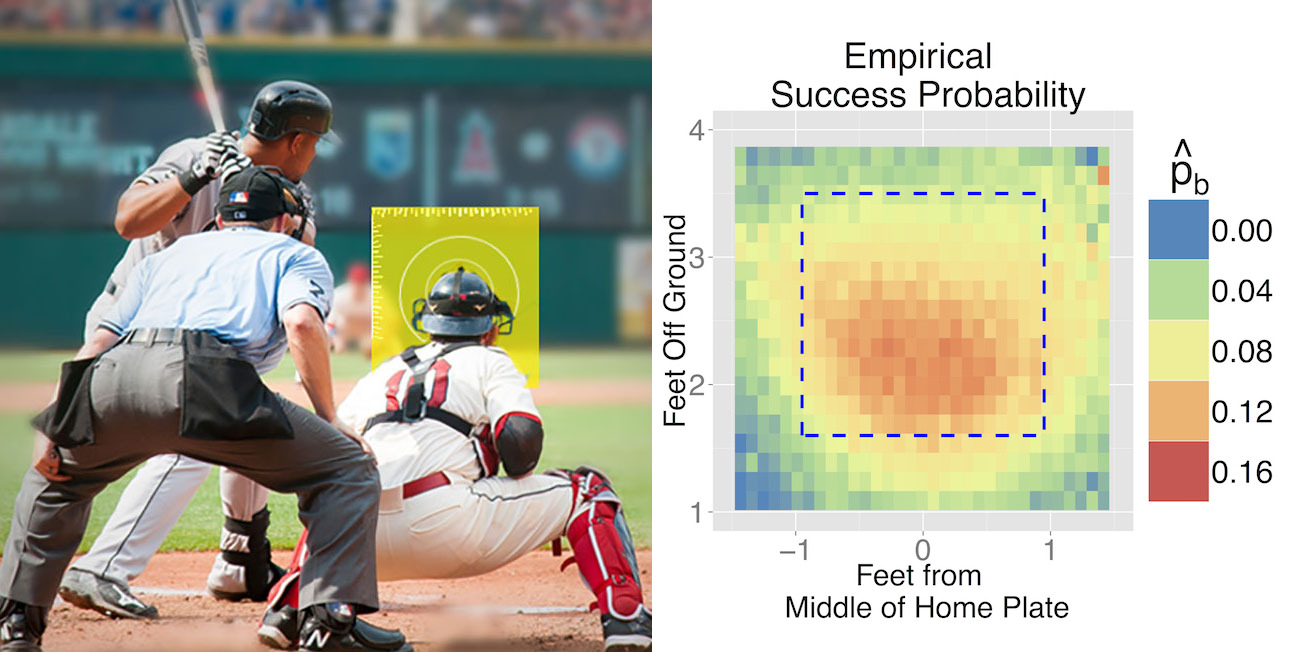
\includegraphics[scale=.35]{Images/SZandMothership.jpg} 
  \caption{The setup, and the heat map. The setup in the image on the left demonstrates the proper perspective for understanding the heat map on the right. This heat map grids the hitting zone with approximately 3/4 inch by 3/4 inch boxes. The dashed blue line on the right outlines, roughly, the yellow box on the left. Each grid box color represents the empirical success probability ($\hat{p}_{b}$) of hitter swings at pitches passing through that box.  The data consists of 1,932 right handed hitters, swinging at 1,582,581 pitches between 2008 and 2015.}
	\end{figure} 
While not sophisticated statistically, the graphic efficiently conveys empirical spatial success probabilities, by mapping the statistic $\hat{p}_{b}$ to the color spectrum. However, note that the statistician---not the data---determines the map's resolution.

\section{Resolution} % ============== =============

A heat map's creator {\it chooses} a resolution, thereby determining a uniform grid box size for the heat map prior to audience viewing. This decision carries consequences; resolution selection influences heat map quality and appearance markedly, in much the same way bin width selection influences histograms. Also, note that heat map resolution fails to convey varying spatial data density through the domain, or the strike zone in our case. Thus, the viewer gets no spatial density information, and therefore no understanding of spatially varying estimate sample sizes, variances, etc. As a rule, heat maps do not communicate this information.

The heat map in Figure 1.1 divided the strike zone into relatively small boxes, because the data supported it. By ``supported it'' we mean the small, spatially specific boxes retained a sample size large enough to prevent unacceptable $\hat{p}_{b}$ variance inflation. Defining ``acceptable'' variance depends on context and objectives. For example, a pitching coach might want estimates accurate to within 10 batting average points, 95\% of the time. This margin of error, 0.02, requires a sample size of 32 when $p_{b} = 0.09$.\footnote{Note that the variance depends on the mean for a Bernoulli random variable.} In contrast to the data set used for Figure 1.1, individual hitter data sets vary dramatically in size; ranging from a single swing to over 10,000 swings. 

To reiterate, the choice of resolution can dramatically affect heat map quality, appearance, and the usefulness of the depicted parameter estimates. The decision usually depends on the size and nature of the data set in question, and its spatial dispersion through the domain. To explore this decision in detail, we look at a heat map for one batter.

\section{Resolution Selection}

In this section, we use batter 425509, a veteran player named Jhonny Peralta, to explore resolution selection and its implications. Our data set includes 9,177 Peralta swings. Peralta's swing data yields the heat map in Figure 2, which divides the central region of the strike zone into 16 equally sized boxes. Each box maps $\hat{p}_{b}$ to a color, and we printed box sample sizes, $n_{b}$, on box centers. We will use box sample sizes to reference them. For example, we will call the box in the lower-left ``box 22.'' (**Note: need to make labels bigger.)
        \begin{figure}[H]
      	\centering
      	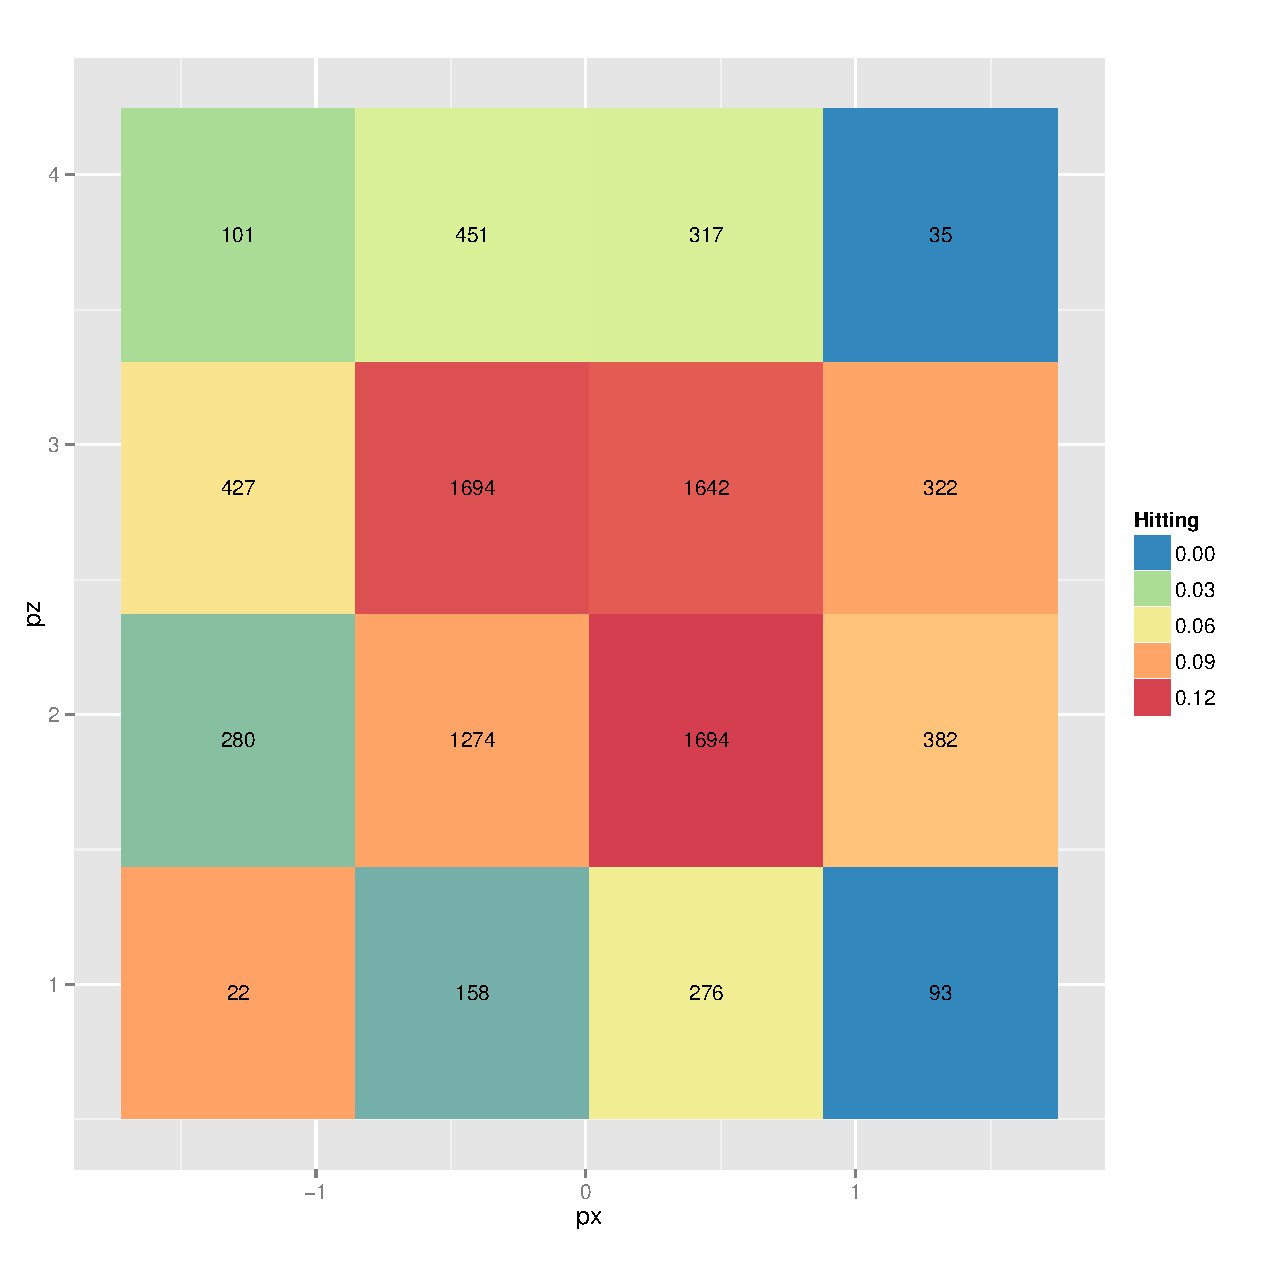
\includegraphics[scale=.35]{Images/Chapter4x4.pdf} 
      	\caption{This four by four heat map shows the empirical batting average of Johnny Peralta, for pitches in each of 16 square regions of the hitting zone. Each box maps $\hat{p}_{b}$ to a color. The number printed on each box gives the number of pitches that Peralta swung at that passed through that box.}
      	\end{figure} 
Why did Peralta see so many fewer pitches in box 22 than in the four center boxes?  We interpret these two box sample sizes in baseball terms for context. Three primary factors influence pitch location: pitcher game theoretic strategy, pitch location margin of error (distance by which a pitch misses its intended target), and game state. Game theoretic strategy concerns the pitcher's knowledge of the hitter's strengths and weaknesses, and the hitter's reciprocal knowledge. Margin of error concerns the pitcher's tendency to miss his intended target by some amount. The game state includes the count (number of balls and strikes), the number of outs, and baserunner presence/absence. Two example game state pressures include the increased penalty for throwing a pitch outside the strike zone on a three ball count (the runner gets on base at four balls); and the increased penalty for a hit with a runner in ``scoring position.'' Our data includes pitches across all game states, so we will not rely on them for interpretation. However, we can use game theory and margin of error rationale. 

Of all low or inside (left-hand side) pitch locations, Peralta enjoyed the most success low and inside, in box 22. The orange color of box 22, compares favorably to the otherwise green, yellow, and blue low or inside pitches. Therefore, we speculate that pitchers simply avoided this location when pitching low or inside. On the other hand, Peralta enjoyed as much or more success in middle of the strike zone, boxes 1694, 1642, 1274, and 1694; and saw and swung at far more pitches there. Why did pitchers not avoid those locations too? They probably tried! However, pitchers often do not have a choice. Game state pressures frequently compel pitchers to throw a strike, and the middle of the strike zone is the most forgiving spot to aim. In addition, Peralta will swing at almost every time the pitcher accidentally throws the easiest pitch to hit.


Why? We can speculate. Box (1,1) pitches often miss the strike zone, because a pitch too low or inside--mistakes in two directions--result in a ball. Or perhaps because hitters typically hit low-inside pitches well. In any event, with $n_{(1,1)}=22$, the four by four resolution sufficiently estimates $\hat{p}_{(1,1)}$; further subdivision would yield trivially small box sample sizes, as we will see. Box (2,3), with $n_{(2,3)} = 1694$ pitches, can support more location specific estimates of $p$ that are still reliable. This motivates finer resolution in that region of space. Peralta succeeds with relatively high probability in Box (2,3), and he probably swings at many pitches in that box. The pitcher knows this, so will seldom aim there. However, by virtue of it location closer to the center of the strike zone, it collects more pitcher mistakes.

Because, as mentioned, box (2,3) sample size justifies a finer resolution, we subdivide all boxes further. For simplicity, without implying we use the only or best subdivision method, we divide each box into four equally sized sub-boxes. Figure 3 shows the eight by eight result.
        \begin{figure}[H]
      	\centering
      	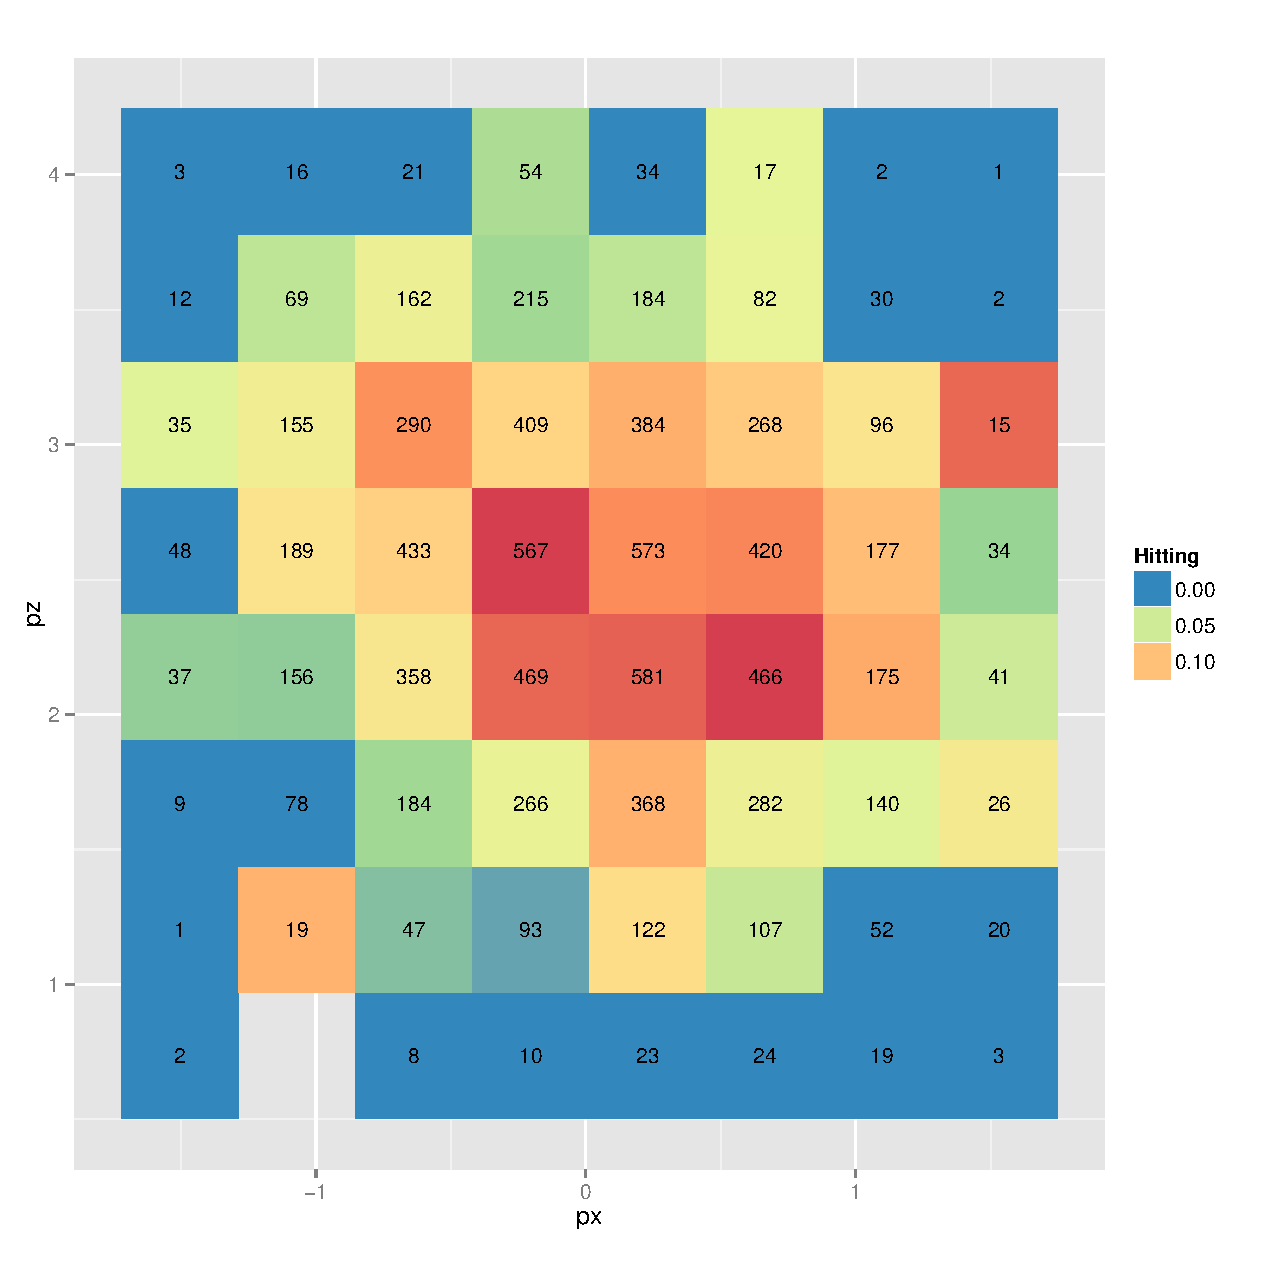
\includegraphics[scale=.25]{Images/Chapter16x16.pdf} 
      	\caption{This eight by eight heat map conveys the empirical batting average of batter 425509, Johnny Peralta, in each of 64 square regions of the hitting zone. Each box maps $\hat{p}_{b}$ to a color. The number printed on each box gives the number of pitches the hitter swung at that passed through that box. A grey box indicates no pitches passed through that box.}
      	\end{figure} 

Boxes (3,5), (3,6), (4,5), and (4,6)---the boxes created by dividing box (2,3) at the four by four resolution---still contain sample sizes sufficient to support low variance $p$ estimates. More generally, 24 boxes still have a sample size greater than 150; and 15 boxes still have a sample size of greater than 250. These boxes could support further subdivision. On the other hand, numerous boxes---corner and edge boxes in particular---now contain sample sizes generally insufficient to support low variance estimates of $p_{b}$. Twenty-nine boxes have a sample size of less than 50, and 17 boxes have a sample size of less than 20. At this resolution one box recorded zero swings.

In this way, due to the particular dispersion of the data, a heat map at any resolution will contain boxes of exceedingly small sample sizes (high variance), and/or boxes of unnecessarily large sample size (unnecessarily low variance). Figure 3 shows six different heat map resolutions, constructed with the same data from Peralta. We started with one box, and subdivided each box into four at each iteration. We chose this simple resolution increasing algorithm to illustrate the resolution selection challenge, and to provide a foundation for our innovation in the next section. 
        \begin{figure}[H]
      	\centering
      	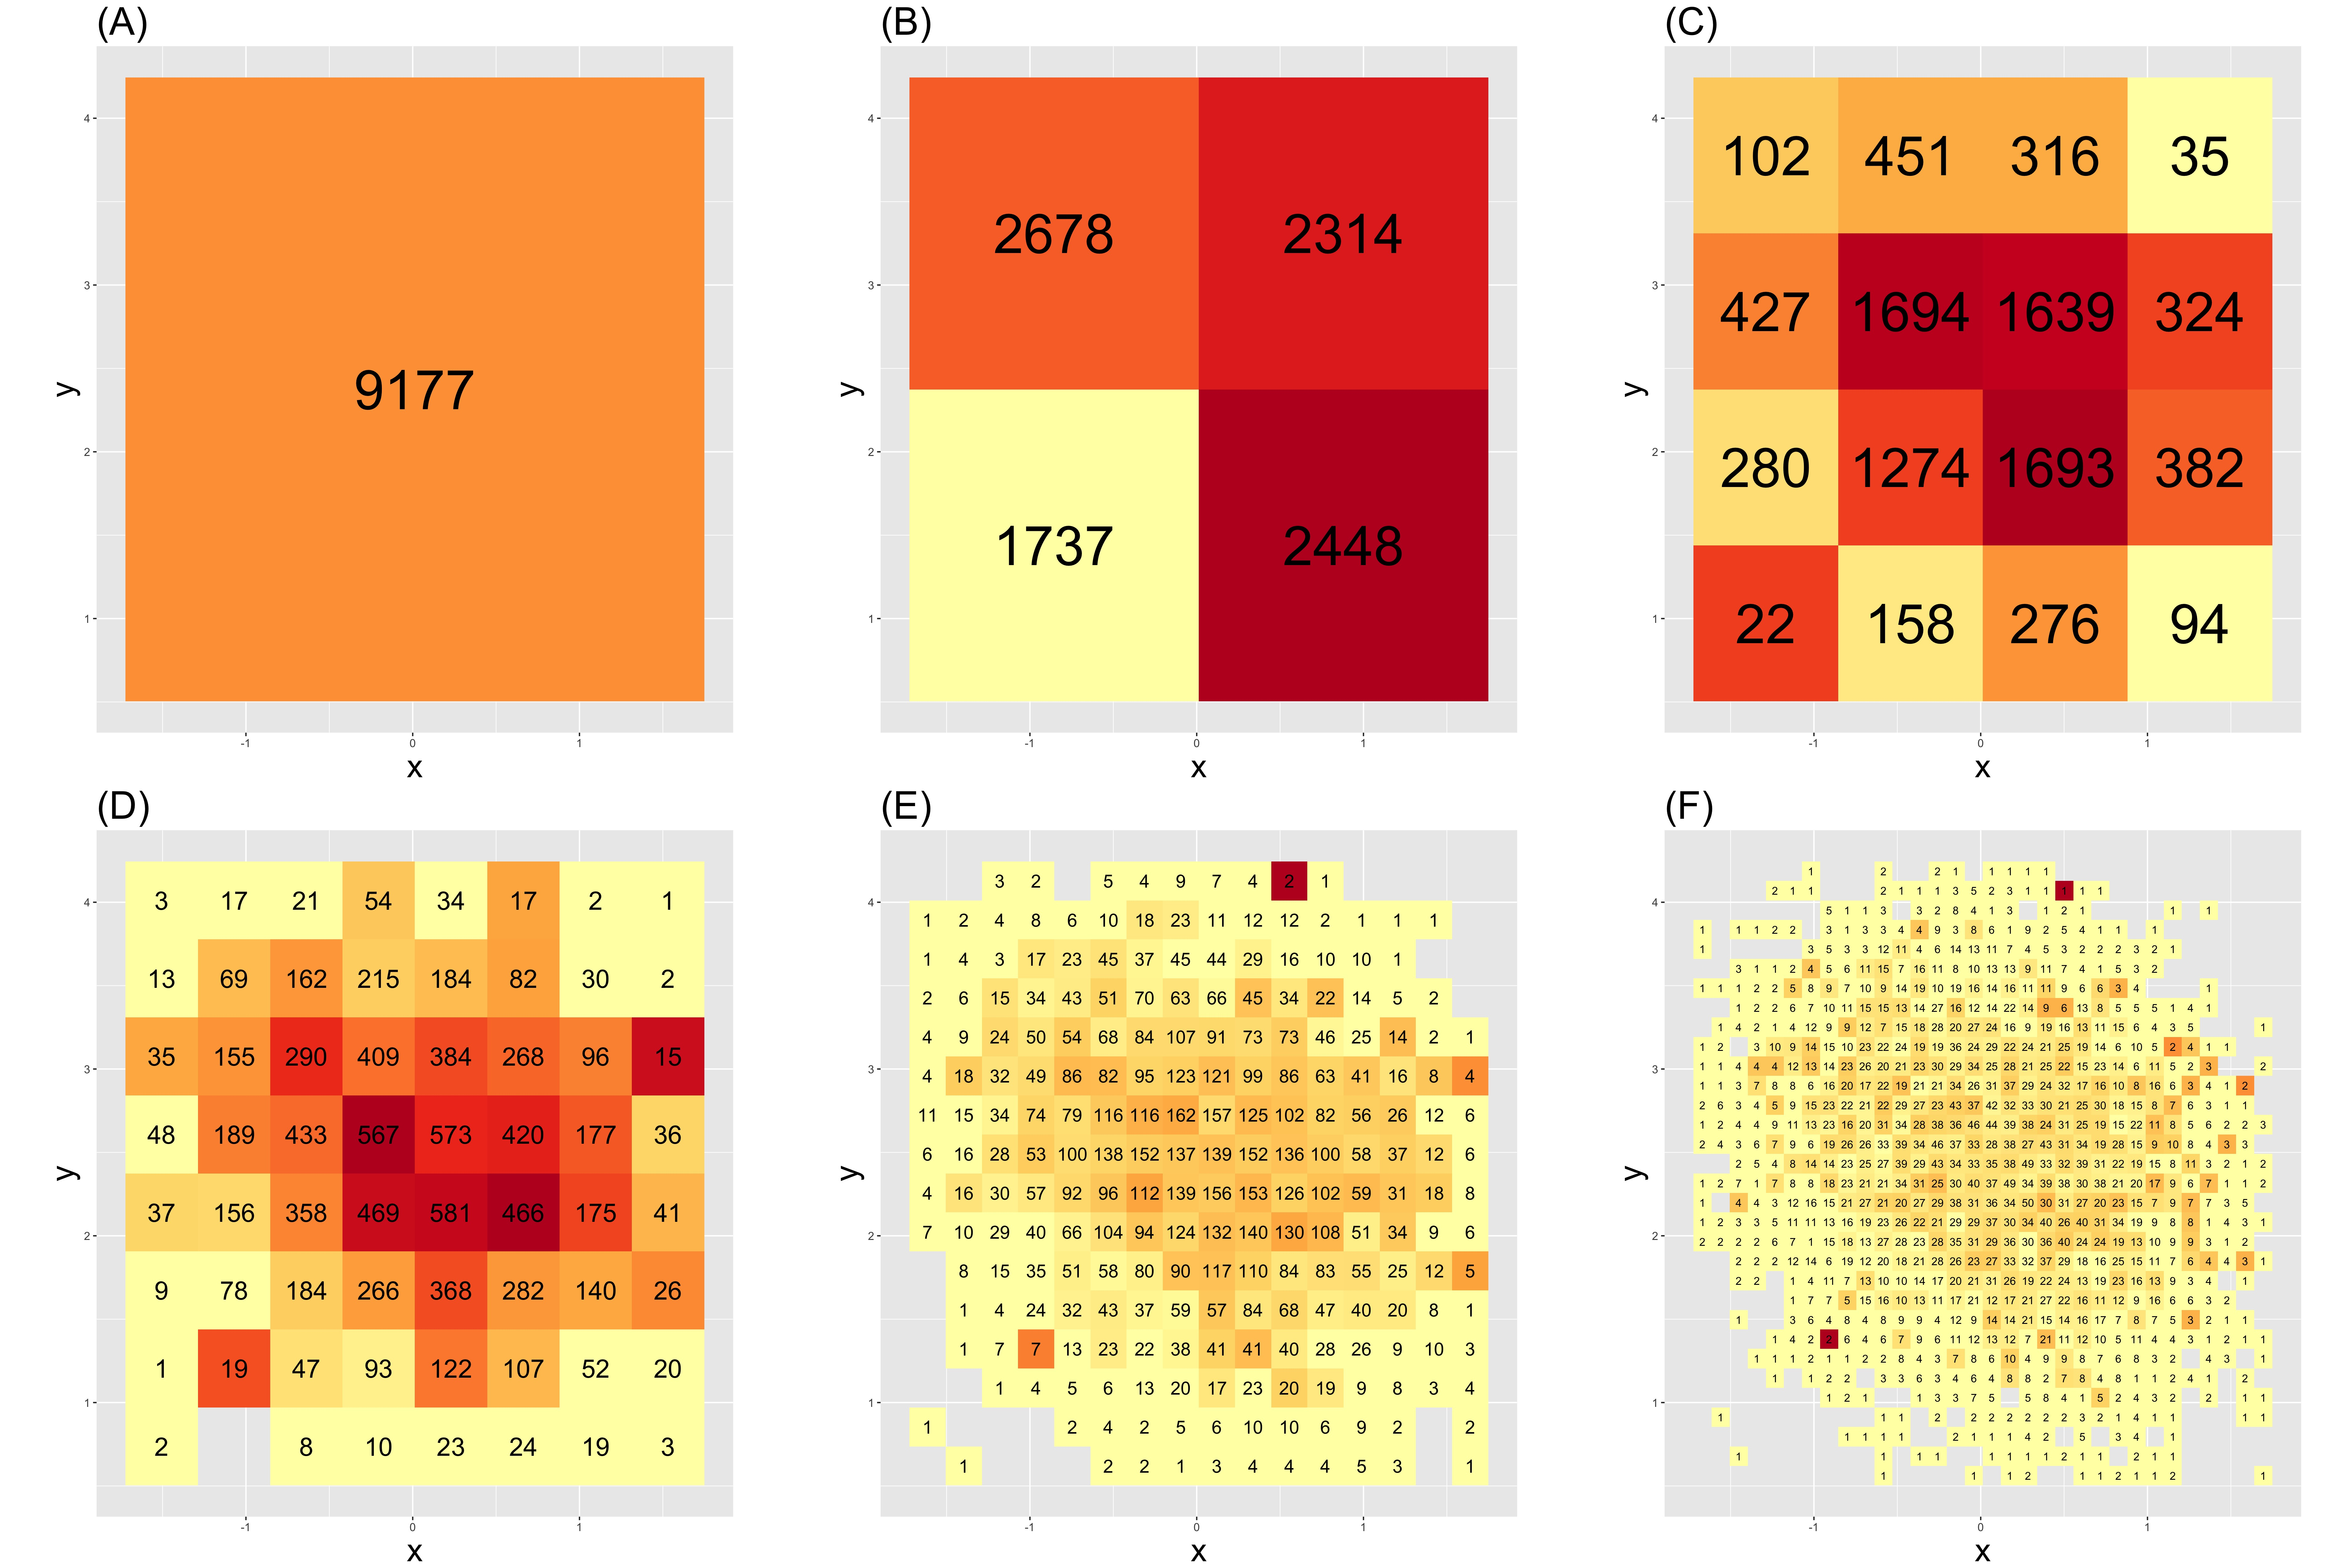
\includegraphics[scale=.4]{Images/Chapter_VarRes.png} 
      	\caption{These {\bf six (?)} heat maps show the same data, 9177 swings by batter 425509, Johnny Peralta, at increasing resolutions. Heat map one is unnecessarily coarse, while heat map six is excessively fine. Note how dramatically the visual impact and impression varies as the resolution increases. Which resolution best conveys the data?}
      	\end{figure} 

It is unclear which of these five resolutions best combines spatially precise estimates of $p$ where possible, and box sample sizes with $\text{Var}(\hat{p}_{b})$ in a desirable range. The viewer interested in the center of the strike zone should prefer the last ({\bf need labels} heat map, as the box sample sizes are sufficient to provide such spatially specific low variance estimates. The boxes closer to the edges of the strike zone contain higher variance, and thus less reliable estimates, due to prohibitively small sample sizes. We propose a new heat map approach that combines resolutions according to the data's varying spatial density.

\section{Spatially Varying Resolution} % ==========

Consider again the heat map in Figure 2. Notice box (1,1) contains data on 22 swings, a sample size where subdividing would yield sample sizes uselessly small, and thus estimate variances prohibitively high. Box (2,3), in contrast, contains data on 1694 swings, which would support estimates that are more spatially accurate without $\text{Var}(\hat{p}_{b})$ increasing past acceptable levels. We propose defining a stopping rule and a subdividing method, and subdividing boxes further accordingly. For example, in Figure 4 we subdivide, into four equally sized boxes, all boxes where $n_{b} > 200$, . One iteration through all boxes at their current size, subdividing according to this rule, converts the heat map on the left to the heat map on the right.
        \begin{figure}[H]
      	\centering
      	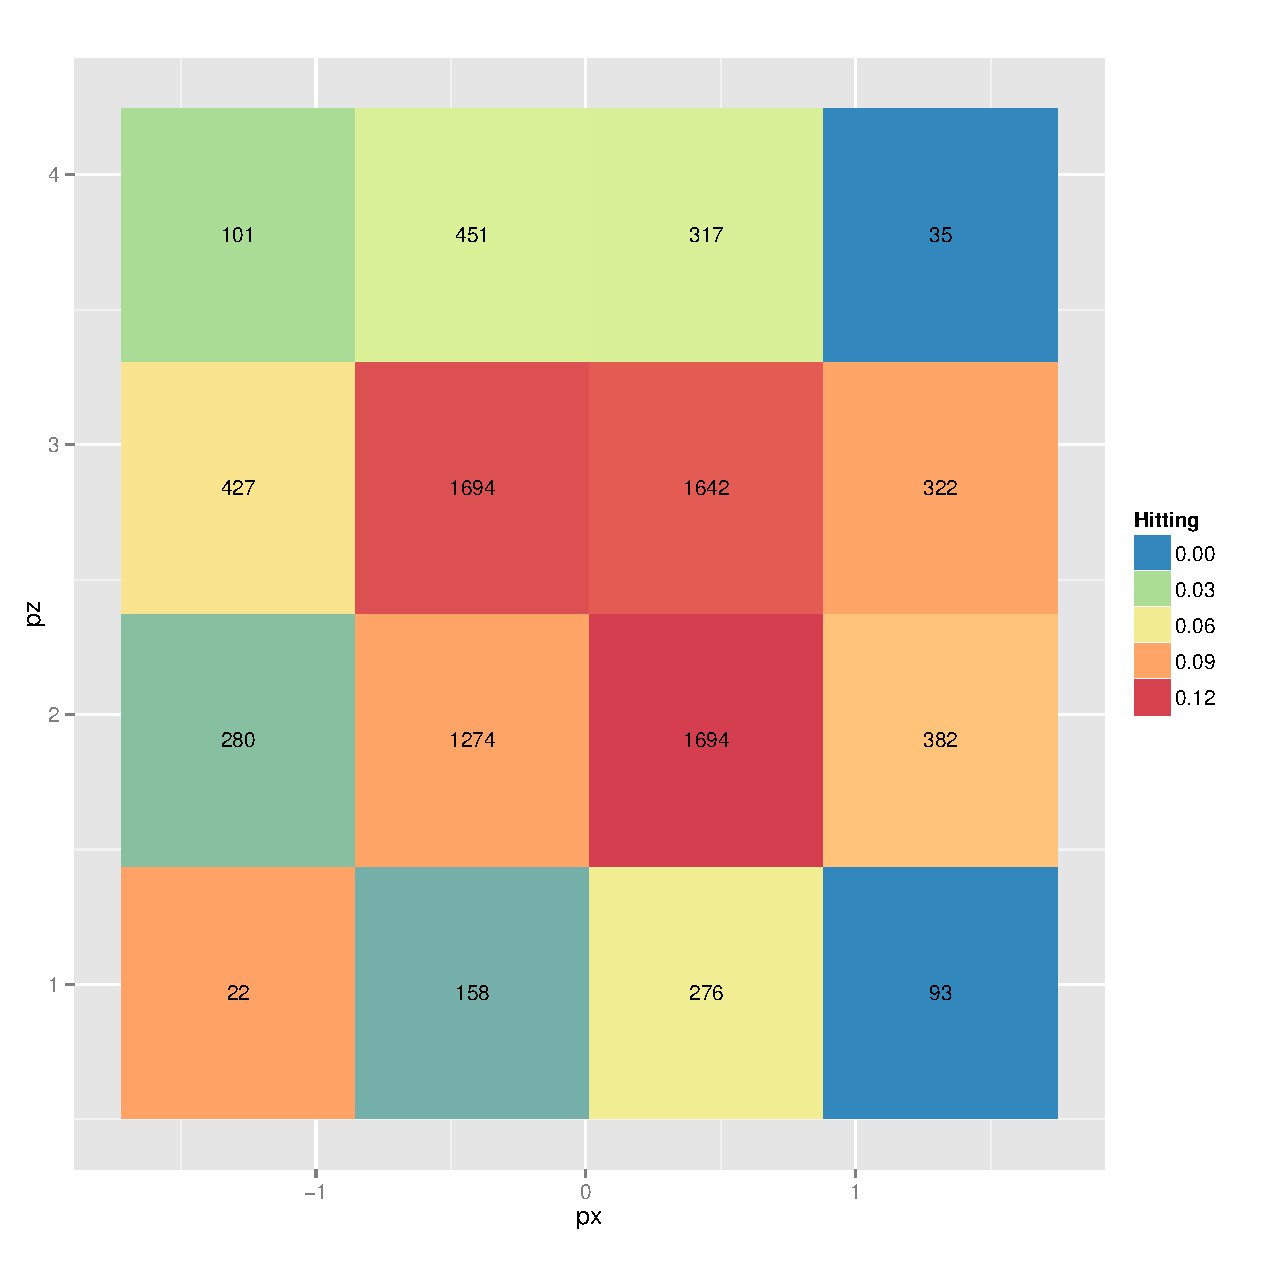
\includegraphics[scale=.3]{Images/Chapter4x4.pdf} 
      	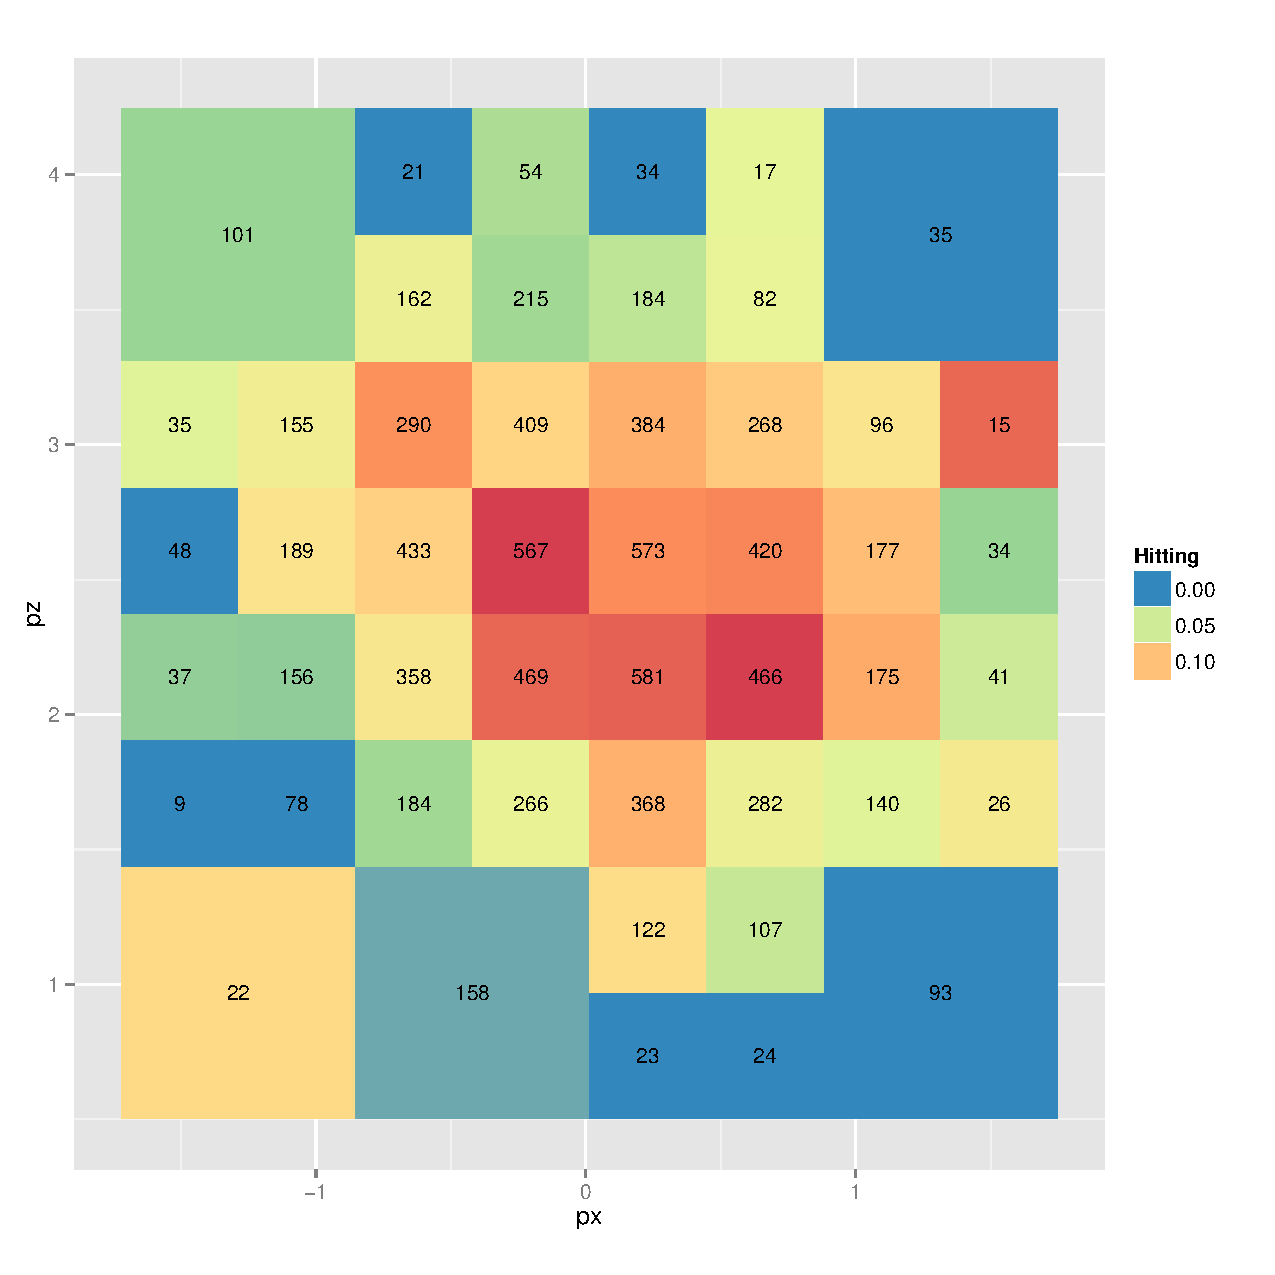
\includegraphics[scale=.3]{Images/Chapter8x8_200.pdf} 
      	\caption{These heat maps convey the empirical batting average of Johnny Peralta in each square region of the hitting zone. Each box maps $\hat{p}_{b}$ to a color. The number printed on each box represents the number of pitches Peralta swung at that passed through that box. Notice that all boxes with a sample size greater than 200 in the heat map on the left, have been subdivided in the heat map on the right.}
      	\end{figure} 
Notice all four corner boxes have not subdivided, indicating Peralta seldom sees and swings at pitches in these locations. The boxes toward the middle of the map tend to have larger sample sizes, and higher $\hat{p}_{b}$. Pitches pass through the middle of the hitting zone more frequently because many pitch target margin of error circles overlap there; and it is the region where pitch target margin of error circles are entirely inside the strike zone. Sixteen boxes still have a sample size greater than 200, and 11 still have a sample size greater than 300. We iterate again, and further subdivide 16 boxes where $n_{b} > 200$.
        \begin{figure}[H]
      	\centering
      	
      	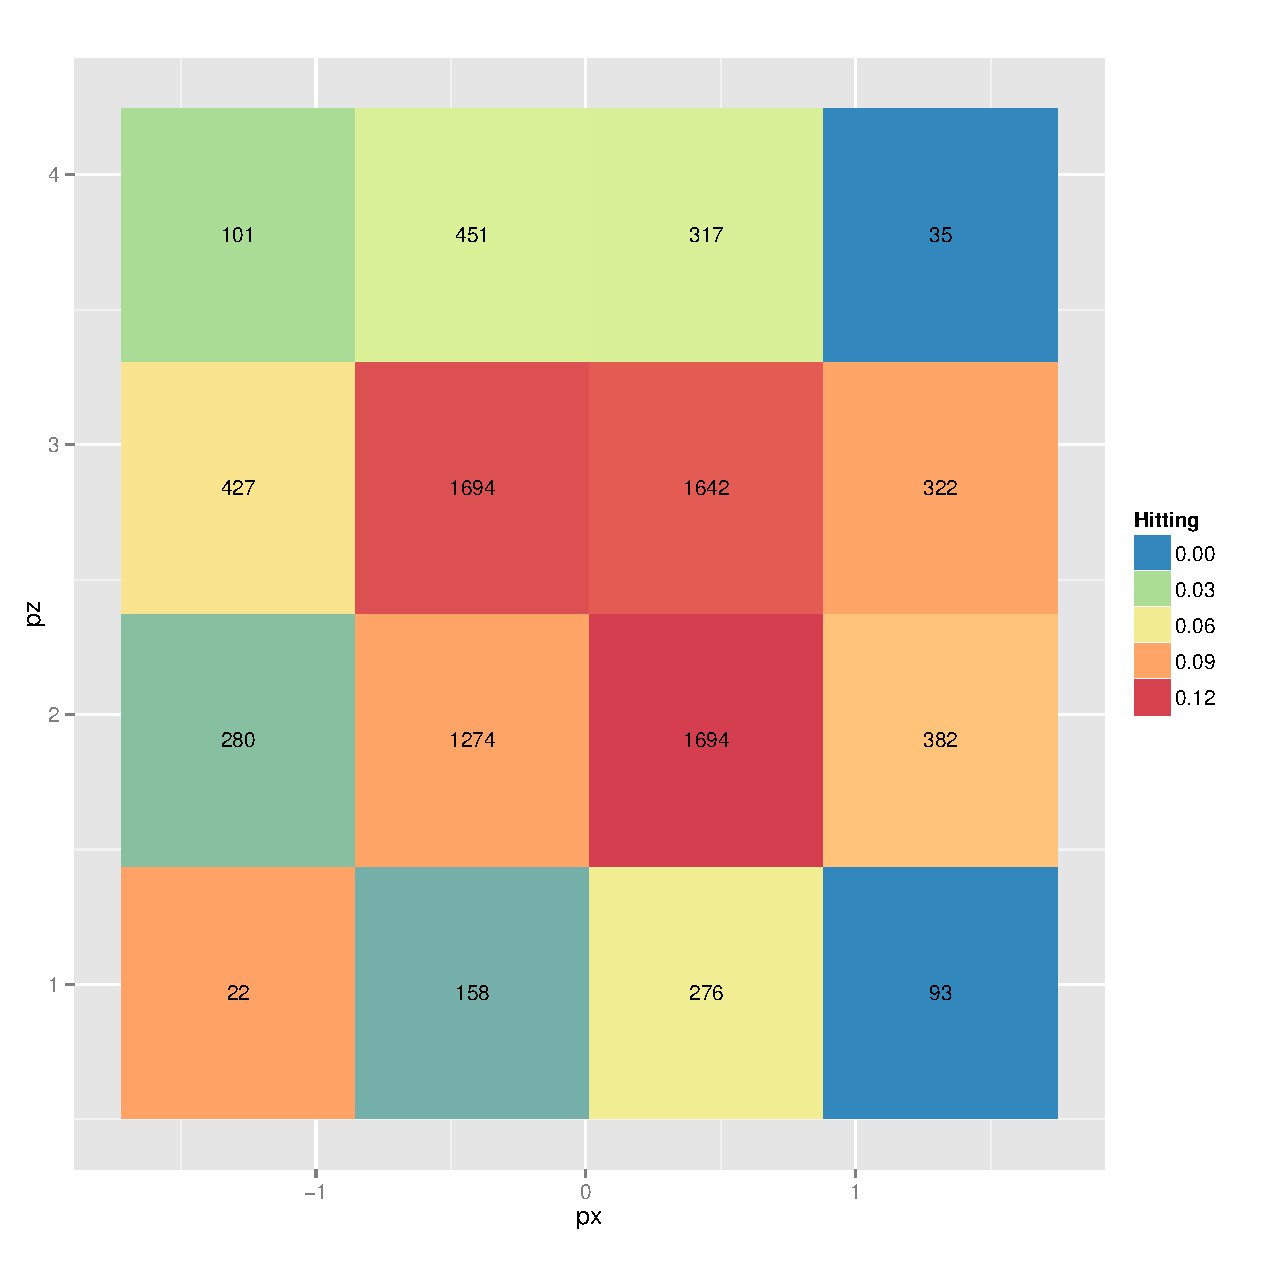
\includegraphics[scale=.25]{Images/Chapter4x4.pdf}
      	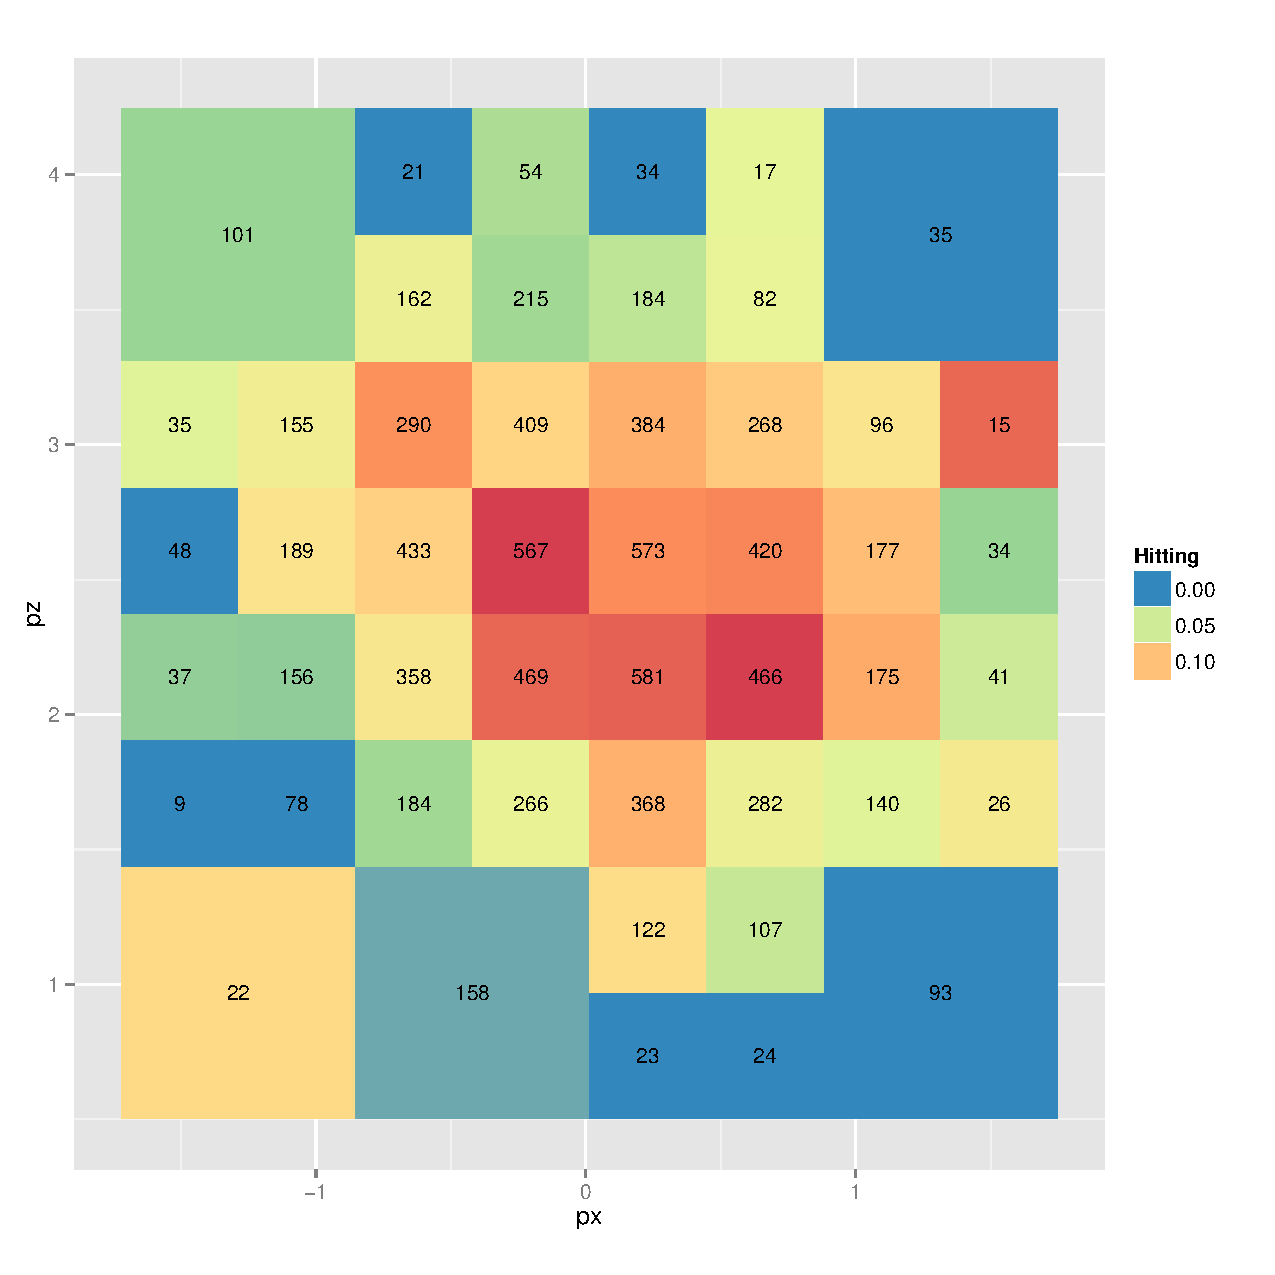
\includegraphics[scale=.25]{Images/Chapter8x8_200.pdf} 
      	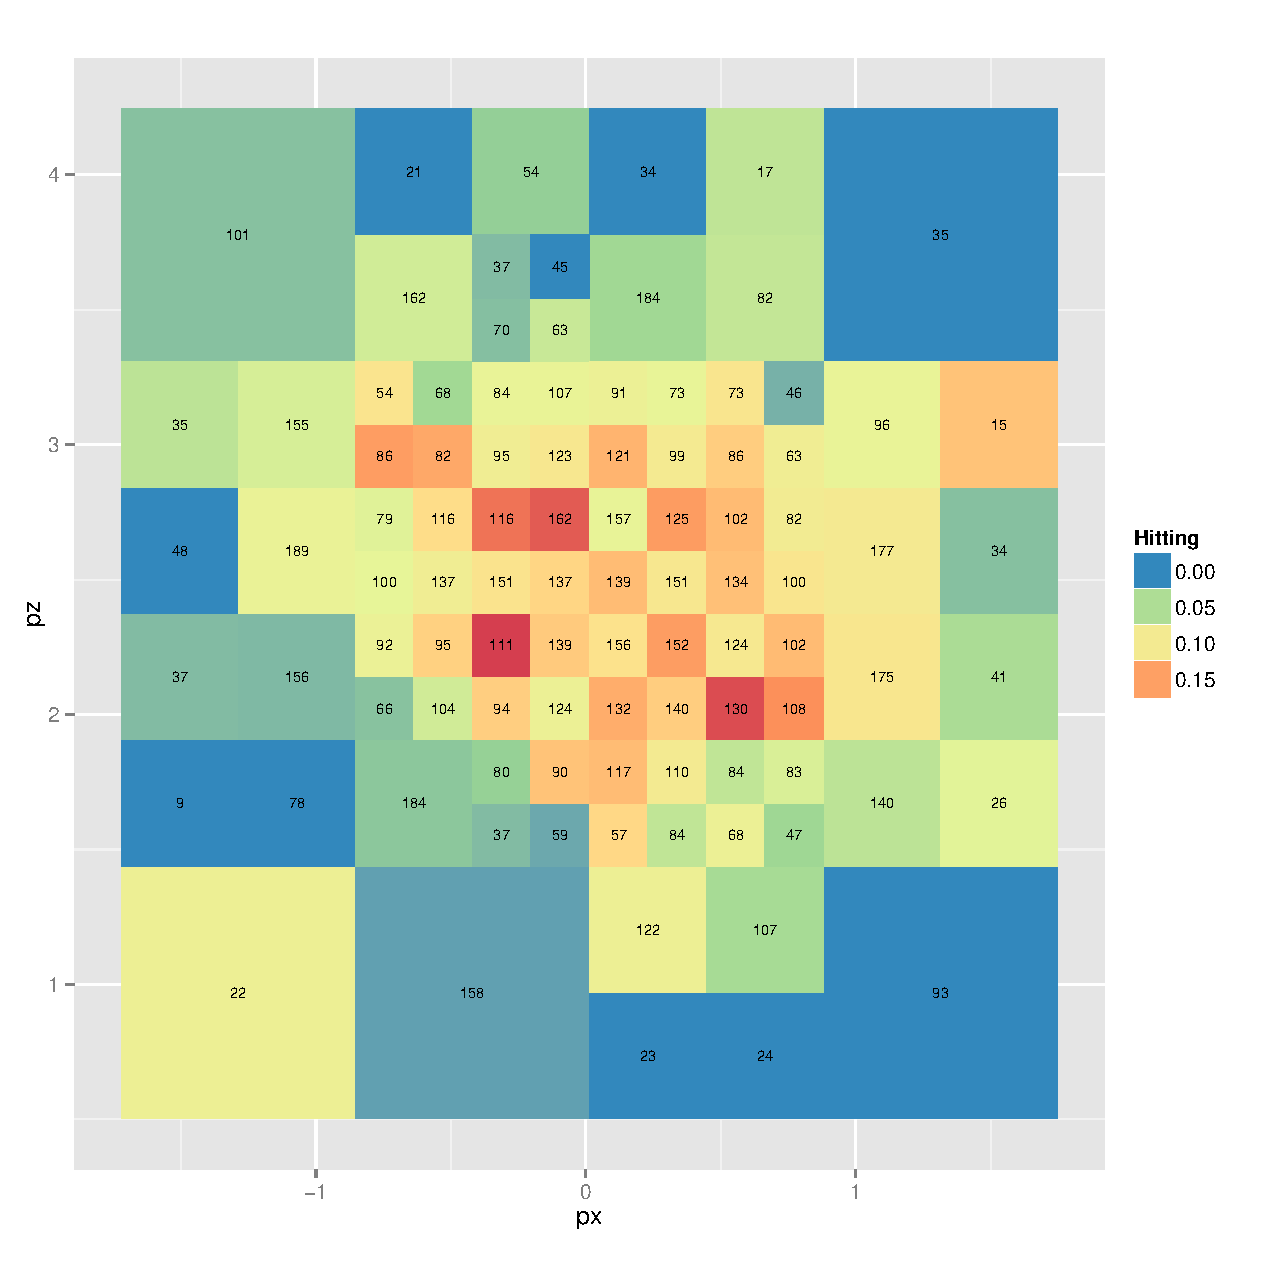
\includegraphics[scale=.25]{Images/Chapter16x16_200.pdf} 
      	\caption{These heat maps convey the empirical batting average of batter 425509, Johnny Peralta, in each boxed region of the hitting zone. Each box maps $\hat{p}_{b}$ to a color. The number printed on each box represents the number of pitches the hitter swung at that passed through that box. All boxes with a sample size greater than 200 in the heat map on the left, have been subdivided in the heat map in the middle. All boxes with a sample size greater than 200 in the heat map in the middle, have been subdivided in the heat map on the right.}
      	\end{figure}
In Figure 6, the middle heat map has 16 boxes with $n_{b} > 200$. In the heat map on the right these 16 boxes have been subdivided into four boxes each. After this iteration, the heat map on the far right consists of 97 boxes, with a mean box sample size of 94.57, and median of 94. The minimum box sample size is 9, and the maximum is 189. The first quartile box sample size is 63, and the third quartile is 125. Regions with a higher density of pitch-swings necessarily have smaller boxes, which acts to convey additional information to the reader, compared to a heat map on a uniform grid. Note that the stopping rule and subdivision algorithm can be defined by the map's creator, offering flexibility to create the heat map structure that suits the data. 

Figure 8 gives the full sequence of heat maps that result from applying the stopping rule $n_{b} < 100$, starting with a single box.
        \begin{figure}[H]
      	\centering
      	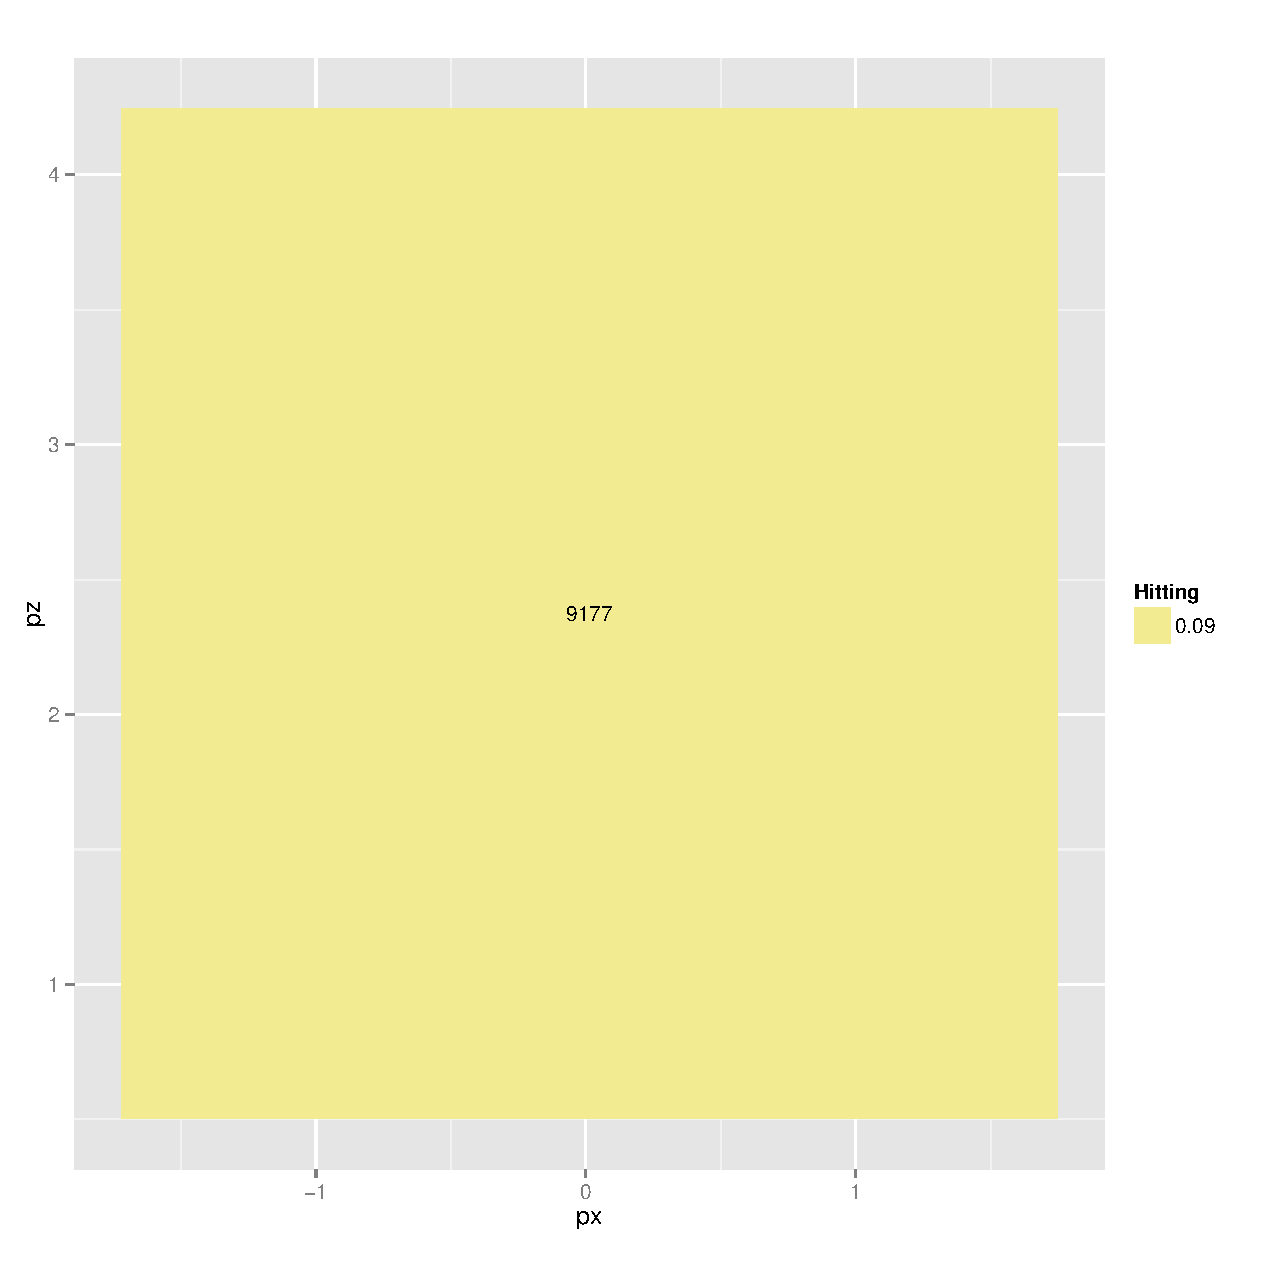
\includegraphics[scale=.2]{Images/Chapter1x1.pdf}
      	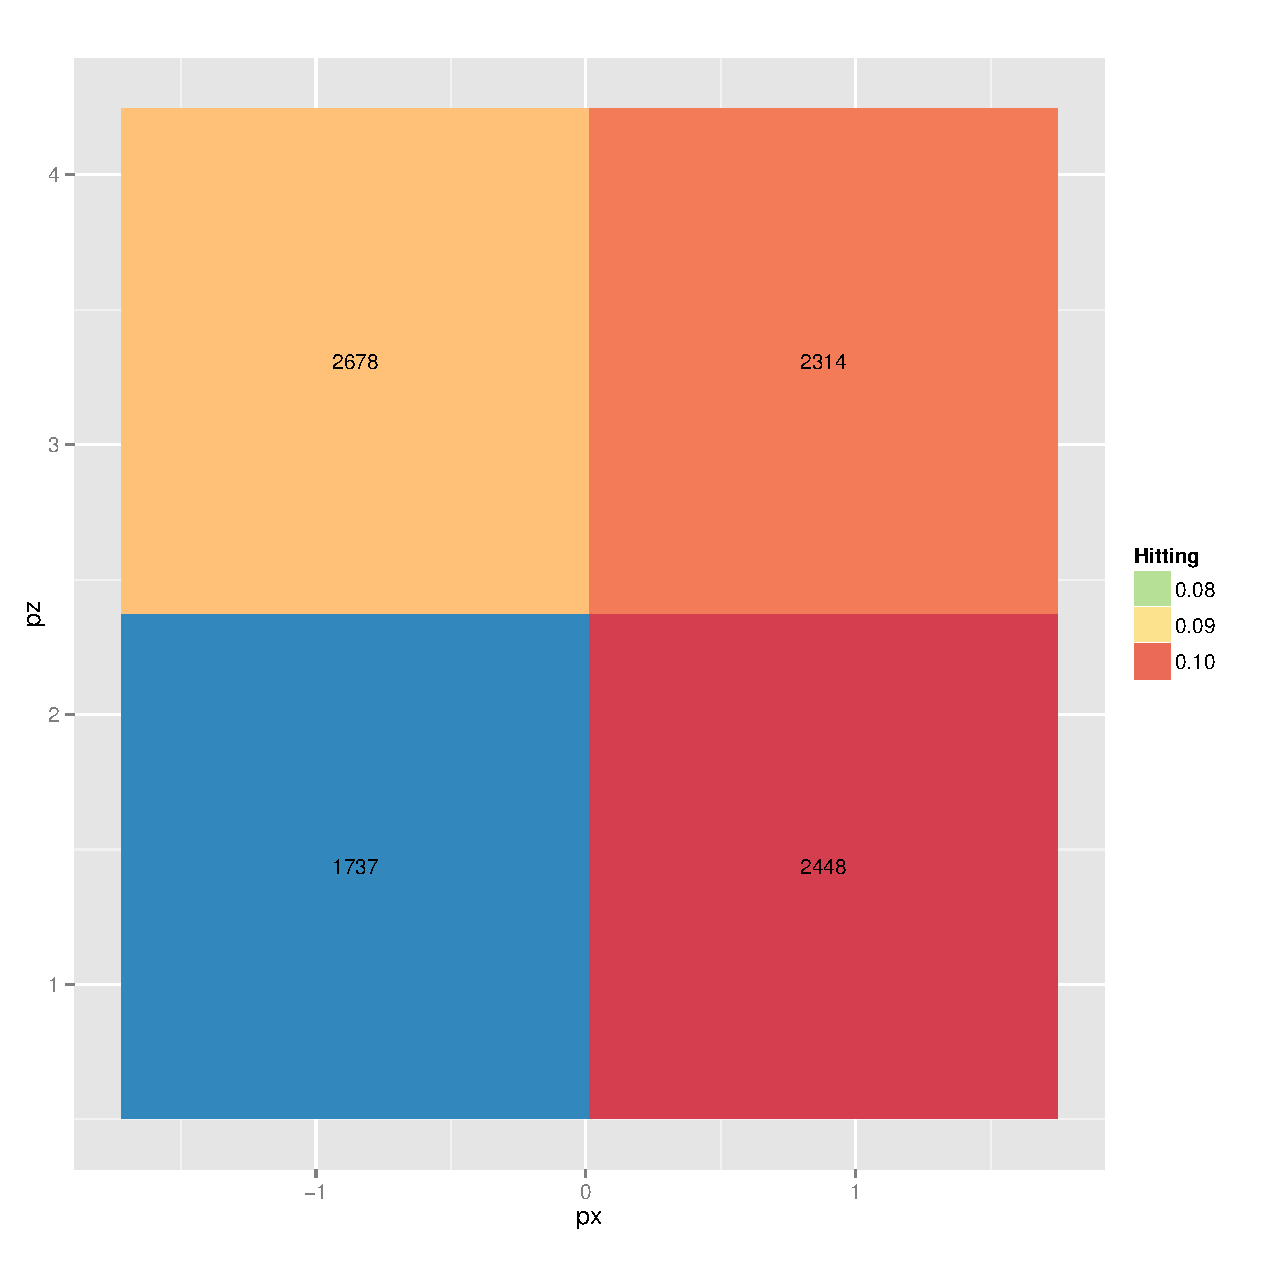
\includegraphics[scale=.2]{Images/Chapter2x2.pdf}
      	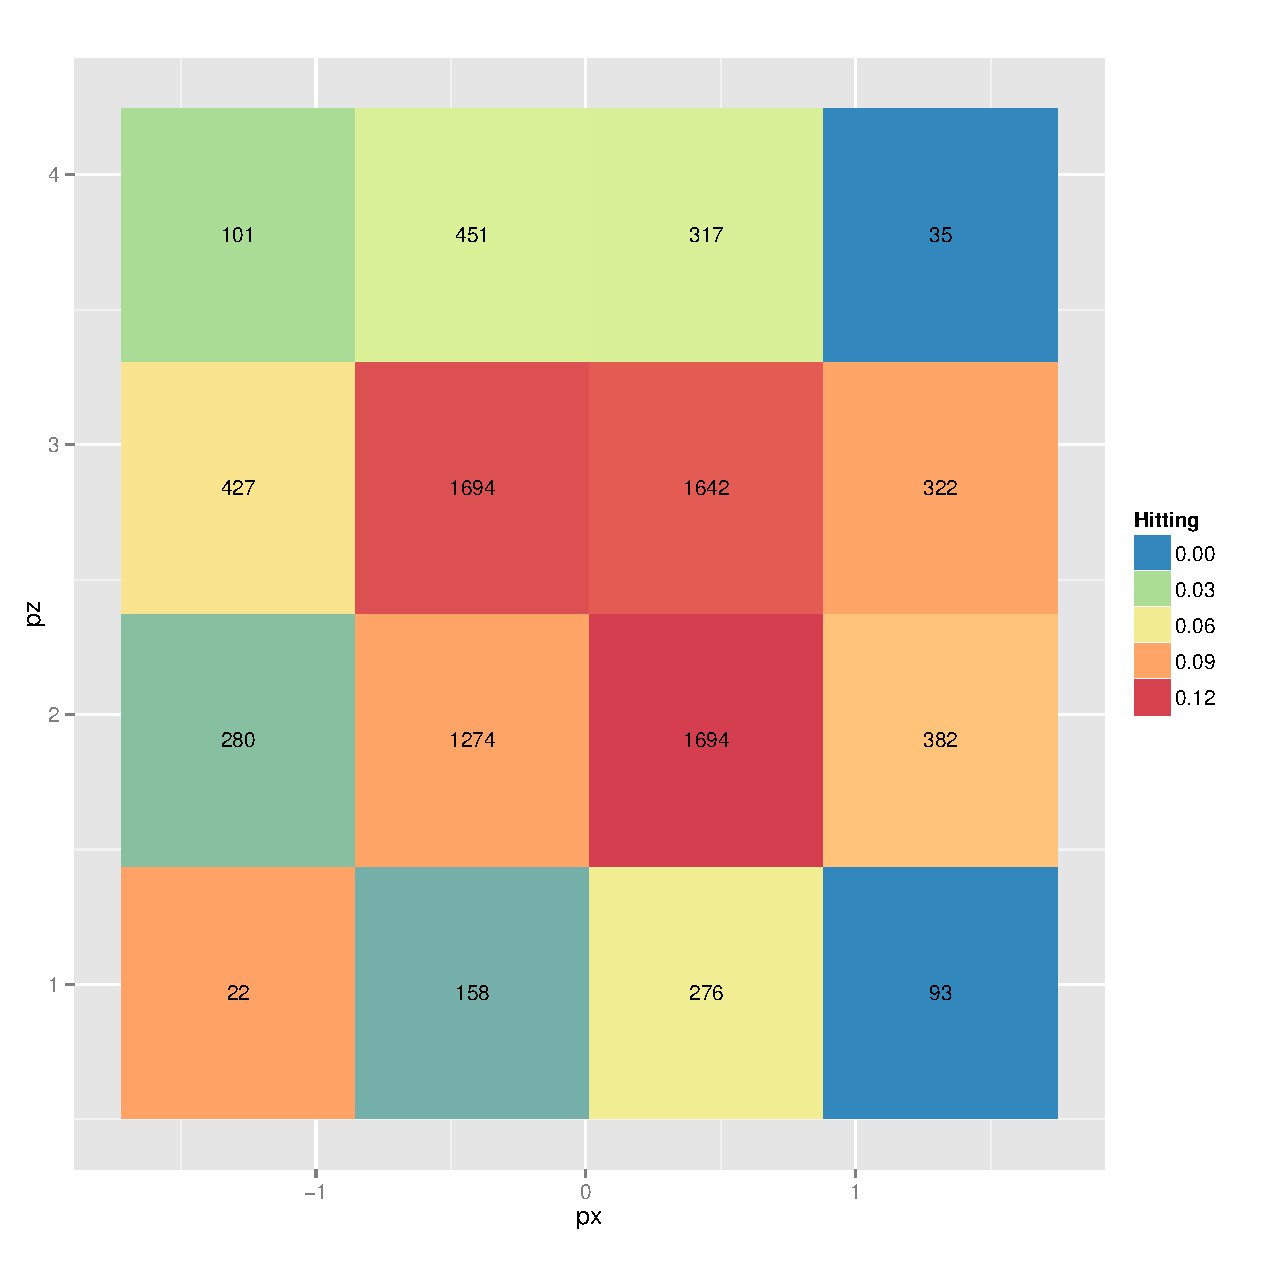
\includegraphics[scale=.2]{Images/Chapter4x4.pdf}
      	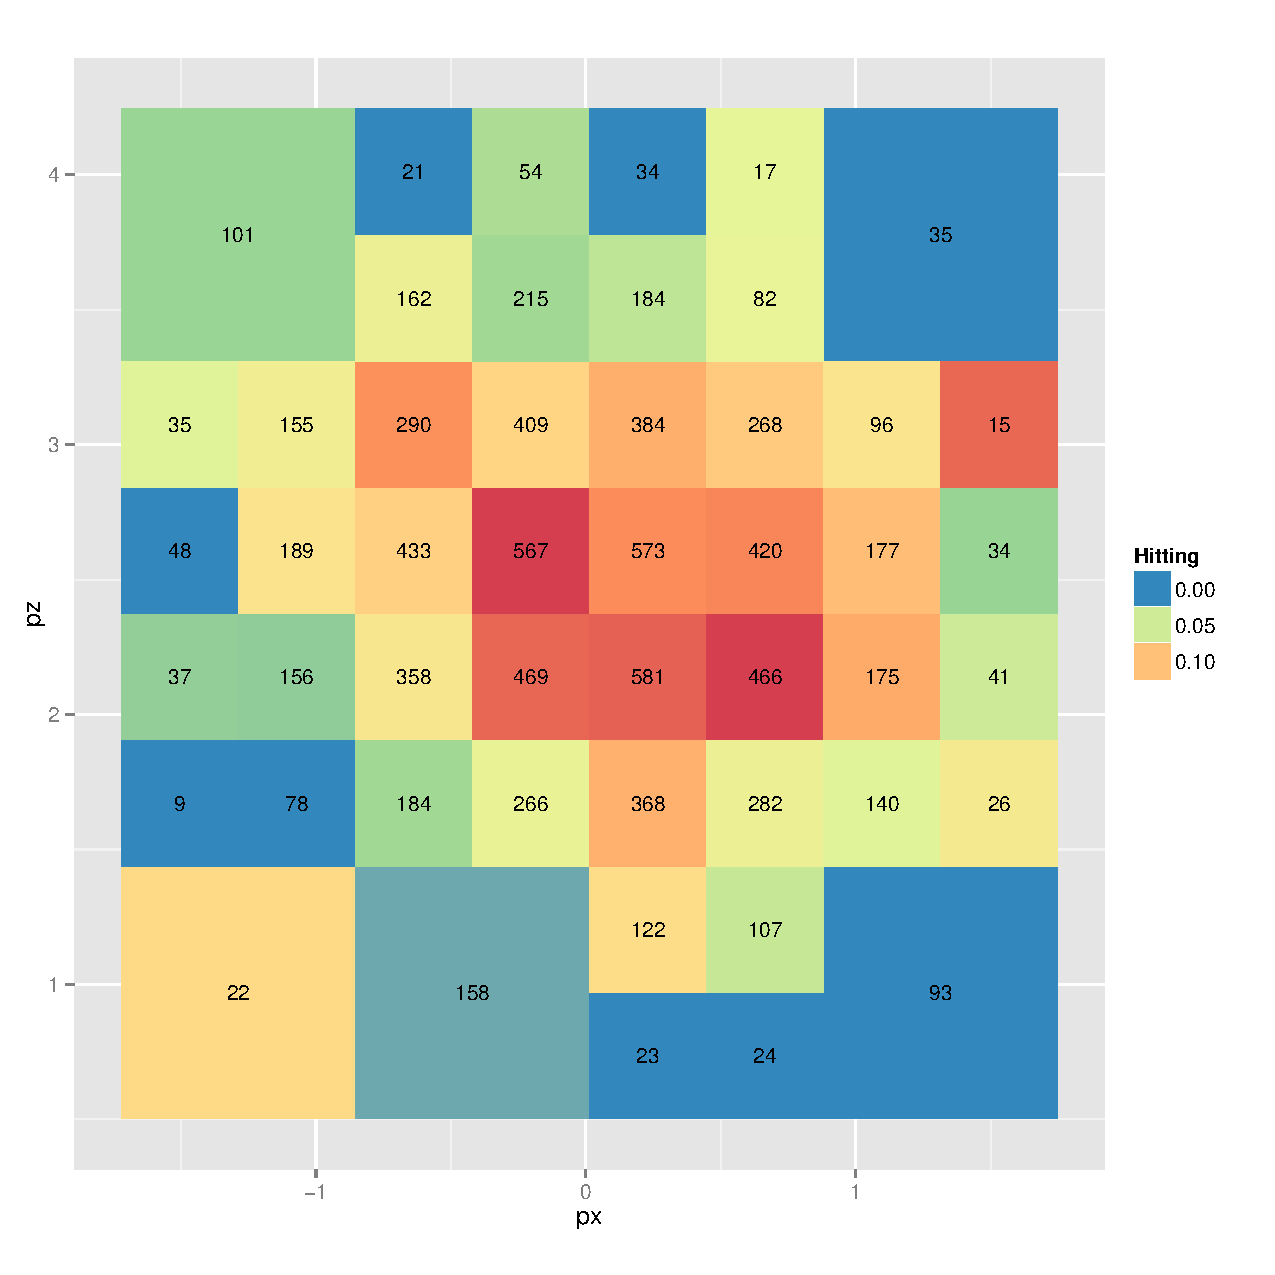
\includegraphics[scale=.2]{Images/Chapter8x8_200.pdf} 
      	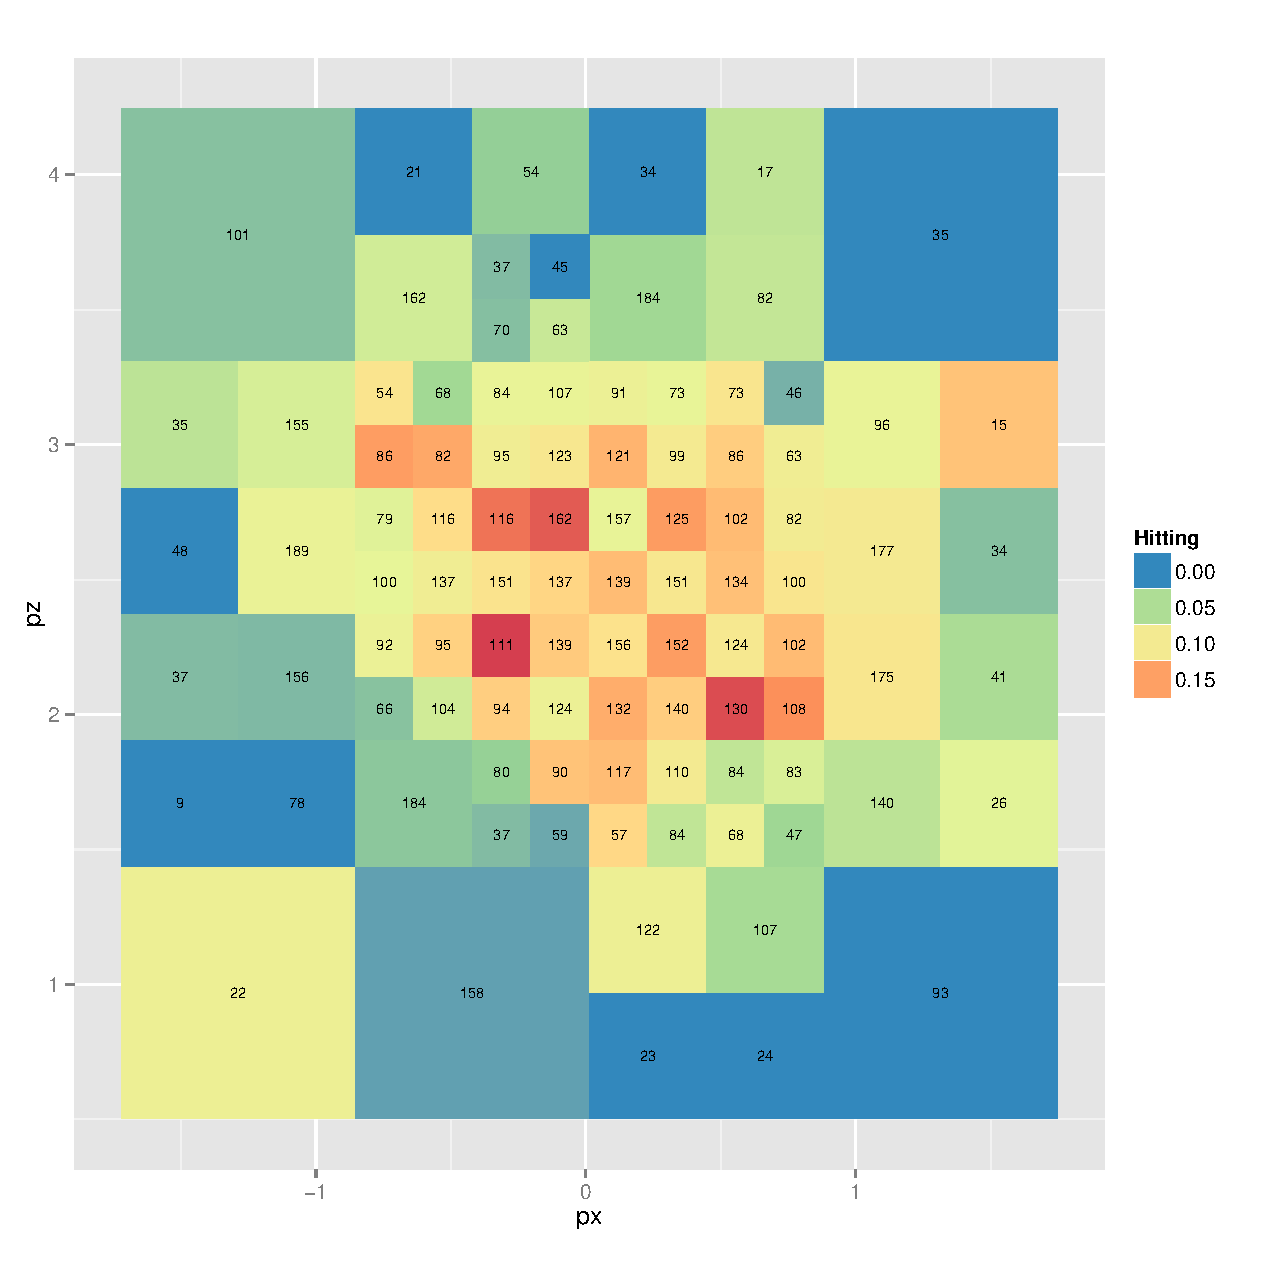
\includegraphics[scale=.2]{Images/Chapter16x16_200.pdf} 
      	\caption{These heat maps convey the empirical batting average of batter 425509, Johnny Peralta, in each boxed region of the hitting zone. Each box maps $\hat{p}_{b}$ to a color. The number printed on each box represents the number of pitches the hitter swung at that passed through that box. All boxes with a sample size greater than 200 in each heat map have been subdivided in the subsequent heat map.}
      	\end{figure}

To demonstrate the flexibility, consider a different stopping rule, $n_{b} < 100$. Figure 8 gives the sequence of heat maps that result from applying this stopping rule, with the same subdividing algorithm (***need to delineate what this algorithm is). 
        \begin{figure}[H]
      	\centering
      	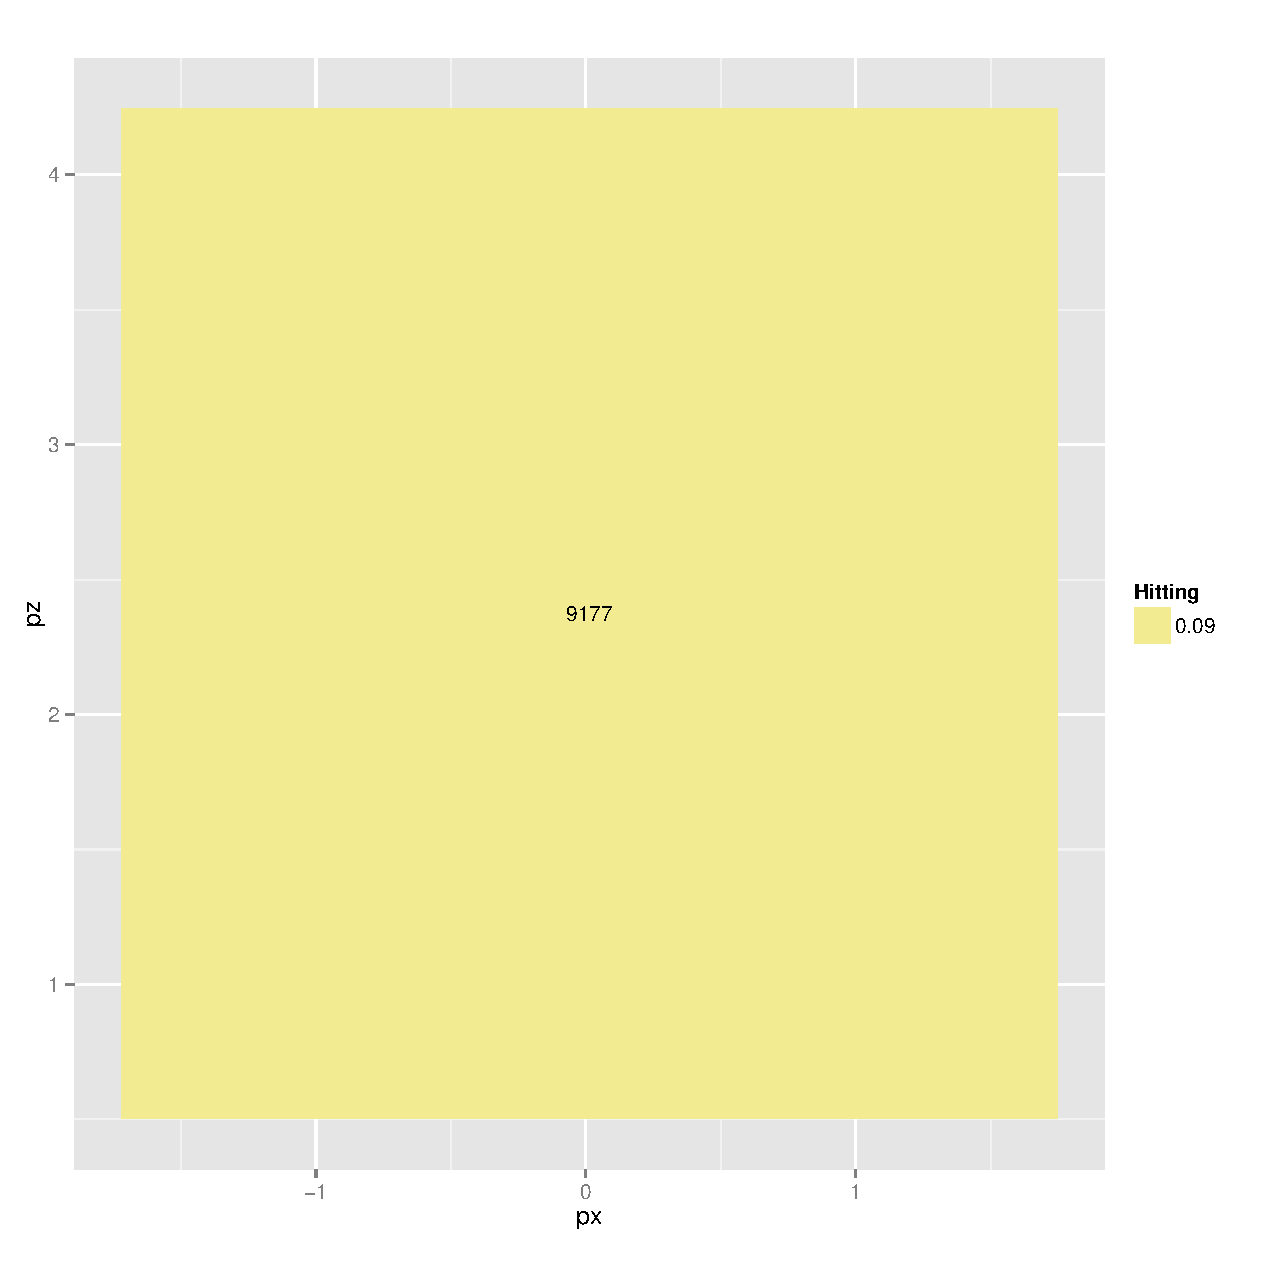
\includegraphics[scale=.2]{Images/Chapter1x1.pdf}
      	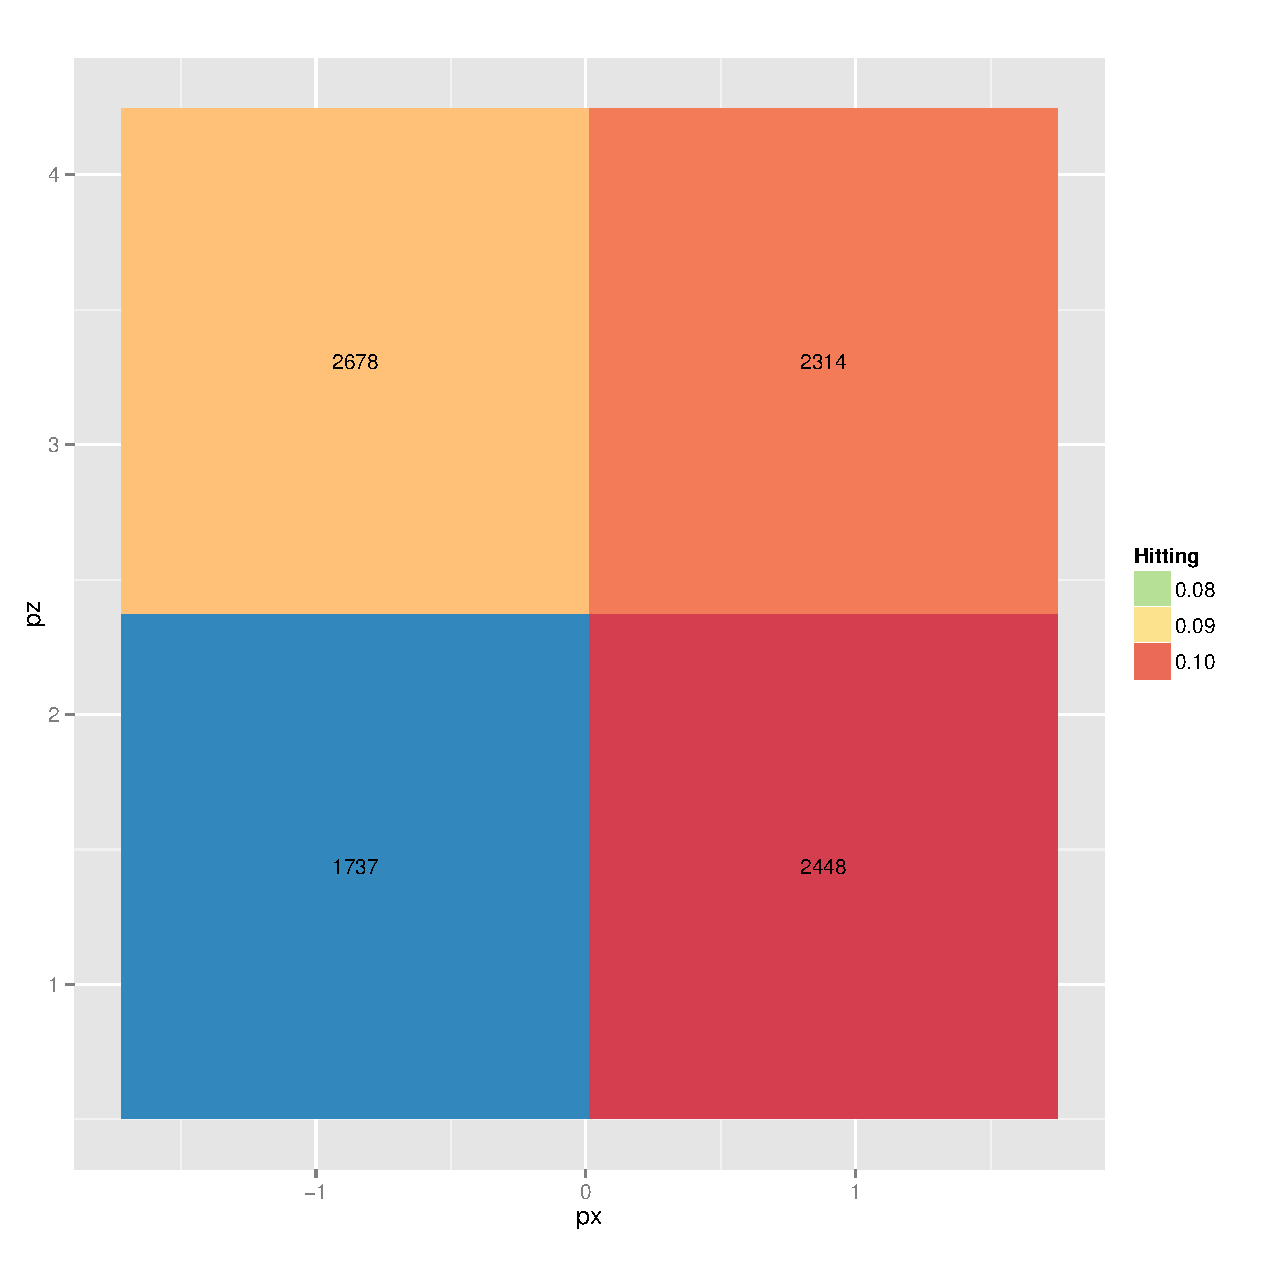
\includegraphics[scale=.2]{Images/Chapter2x2.pdf}
      	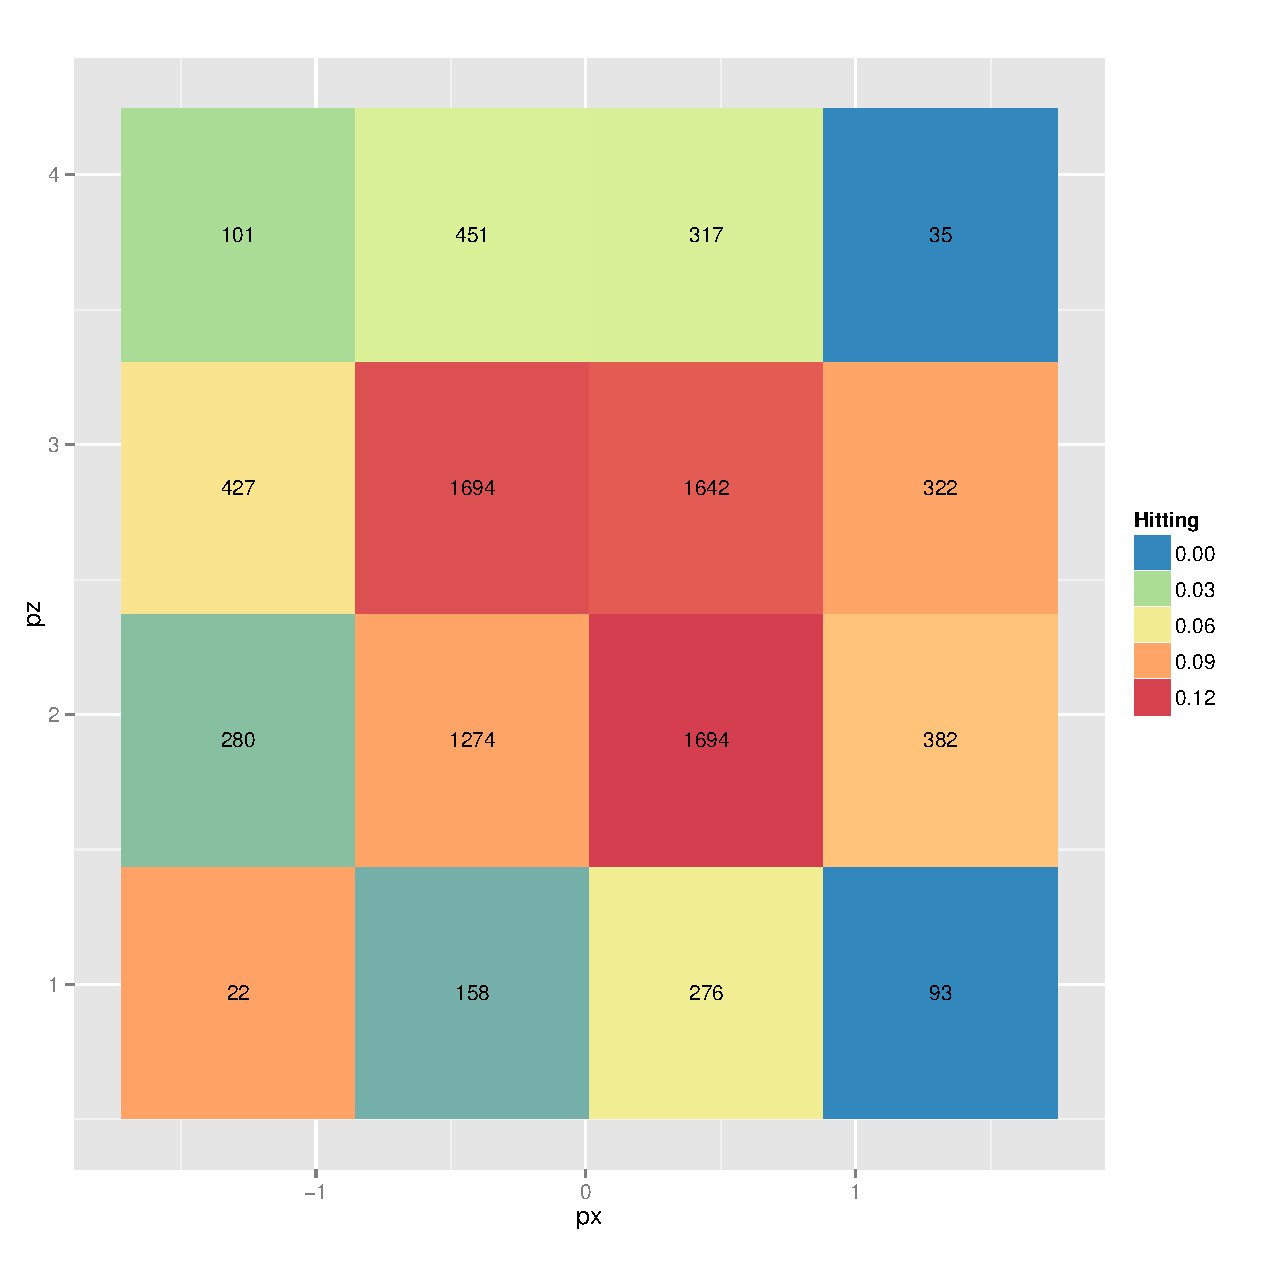
\includegraphics[scale=.2]{Images/Chapter4x4.pdf}
      	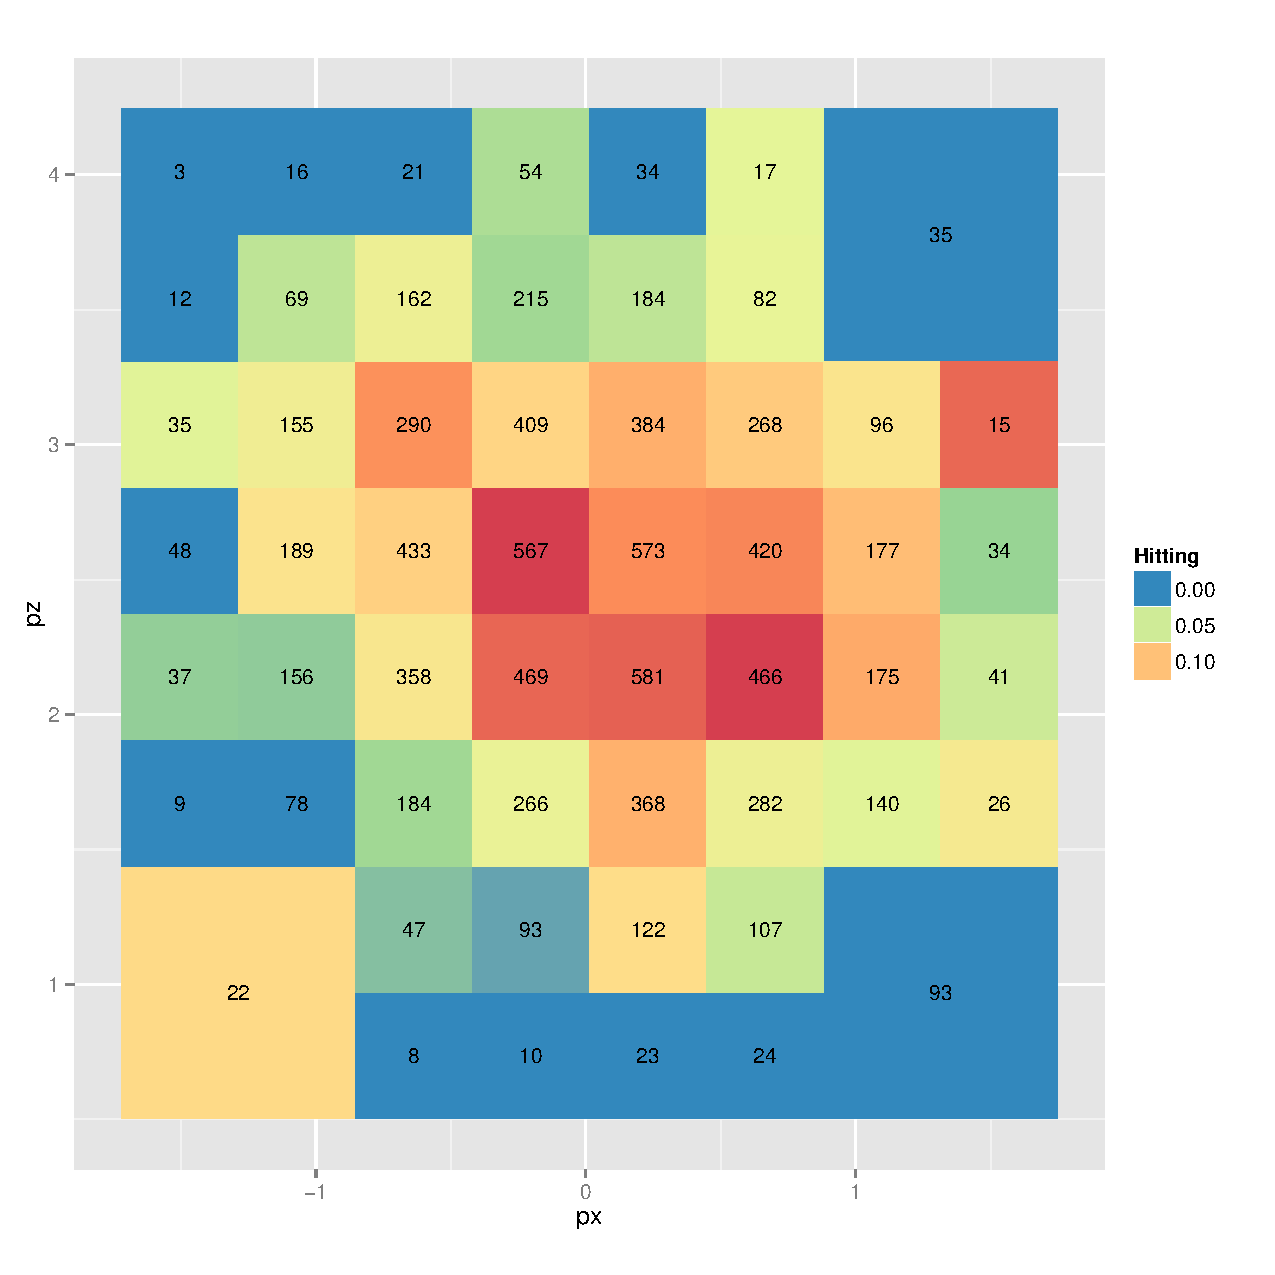
\includegraphics[scale=.2]{Images/Chapter8x8_100.pdf}
      	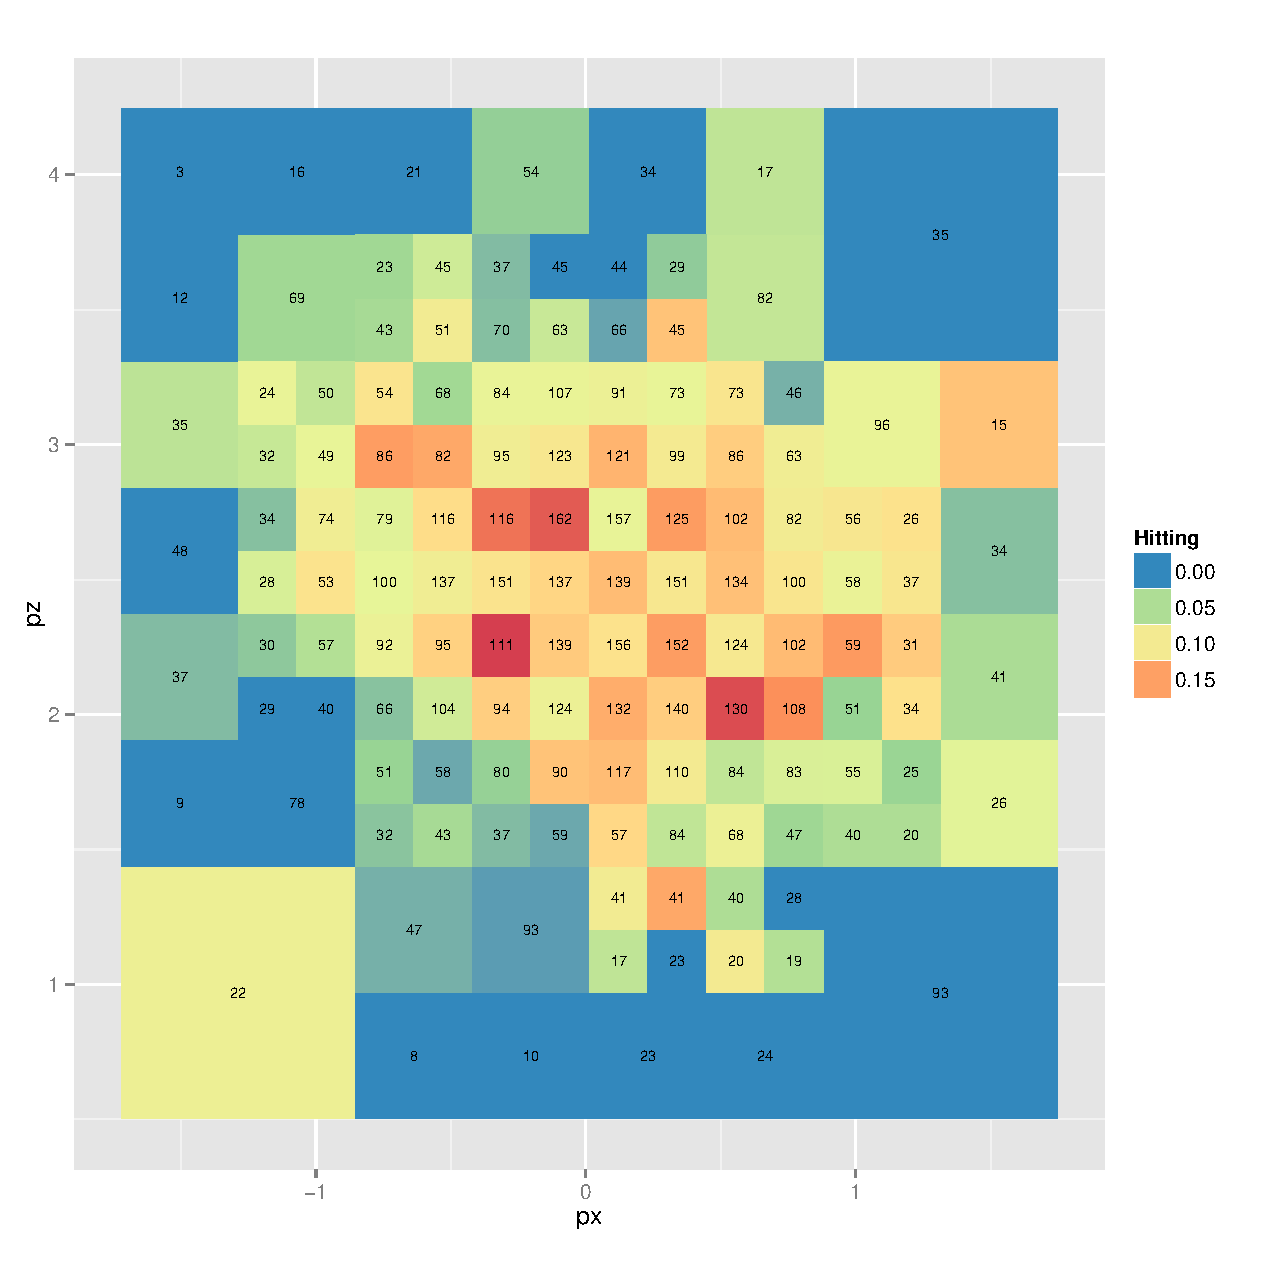
\includegraphics[scale=.2]{Images/Chapter16x16_100.pdf}
      	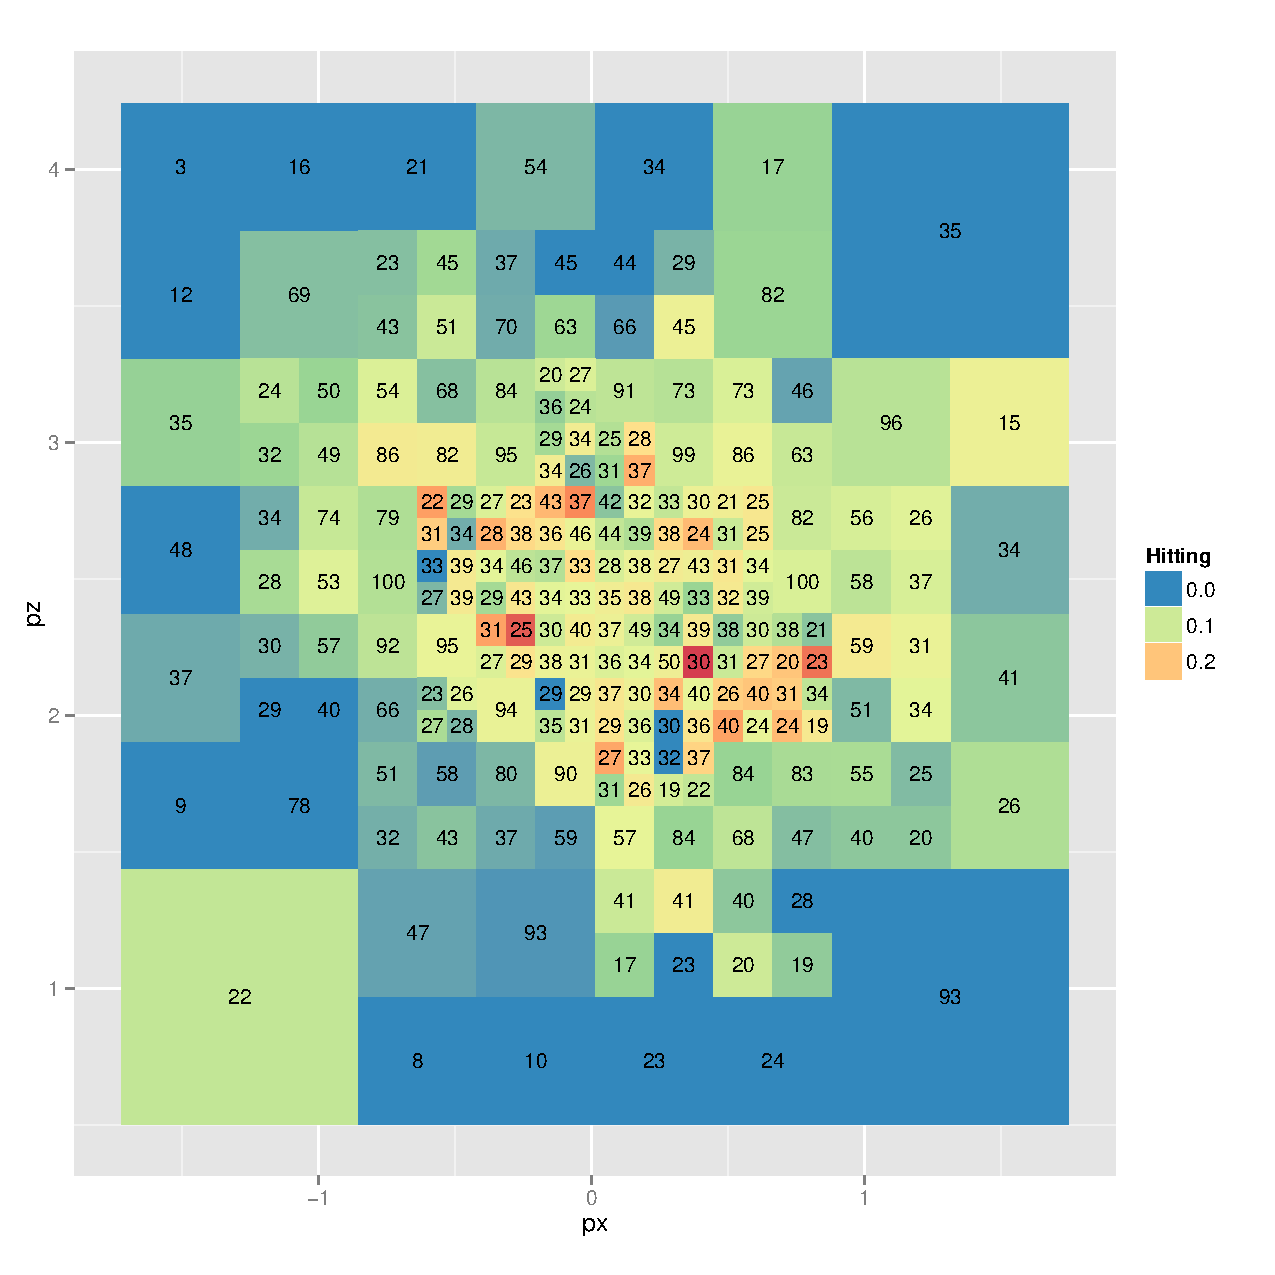
\includegraphics[scale=.2]{Images/Chapter32x32_100.pdf}
      	\caption{These heat maps convey the empirical batting average of batter 425509, Johnny Peralta, in each boxed region of the hitting zone. Each box maps $\hat{p}_{b}$ to a color. The number printed on each box represents the number of pitches the hitter swung at that passed through that box. All boxes with a sample size greater than 100 in each heat map have been subdivided in the subsequent heat map.}
\end{figure} 	
Compare this sequence to Figure 7, where the stopping rule was $n_{b} < 100$. The top row of heat maps in Figure 7 and Figure 8 are identical, but notice in the four by four heat map that $100 < n_{(2,1)} < 200, \text{ and } 100 < n_{(1,4)} < 200$. This implies one stopping rule applies, but the other does not.
        \begin{figure}[H]
      	\centering      
      	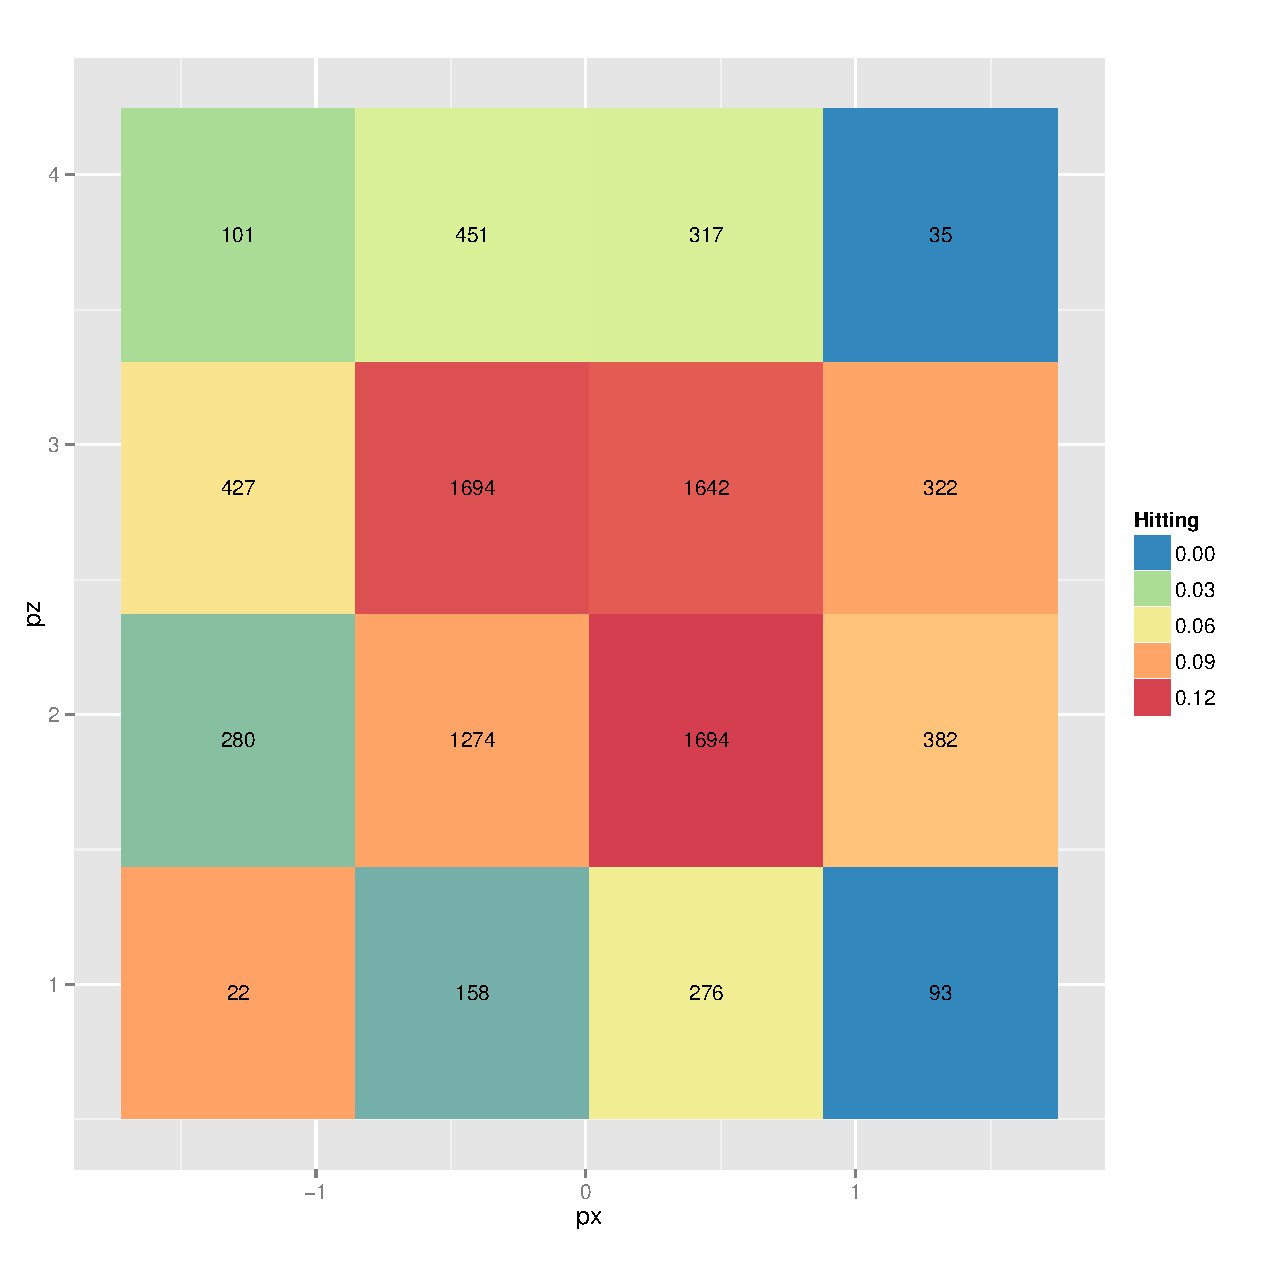
\includegraphics[scale=.2]{Images/Chapter4x4.pdf}
      	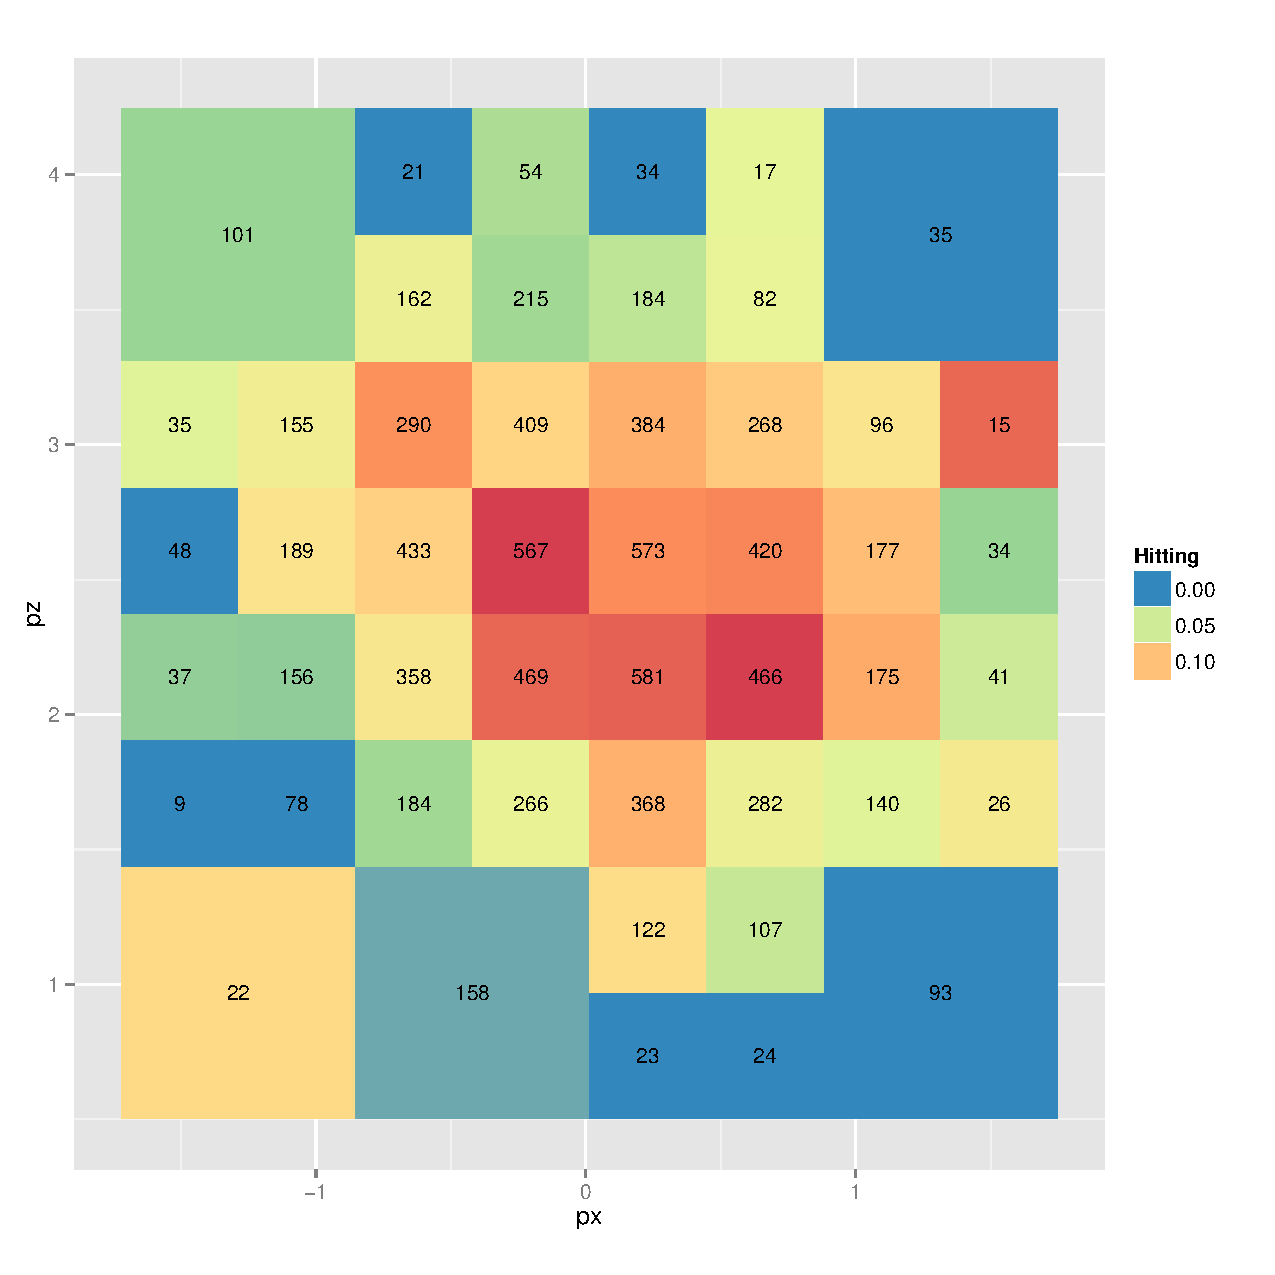
\includegraphics[scale=.2]{Images/Chapter8x8_200.pdf}
      	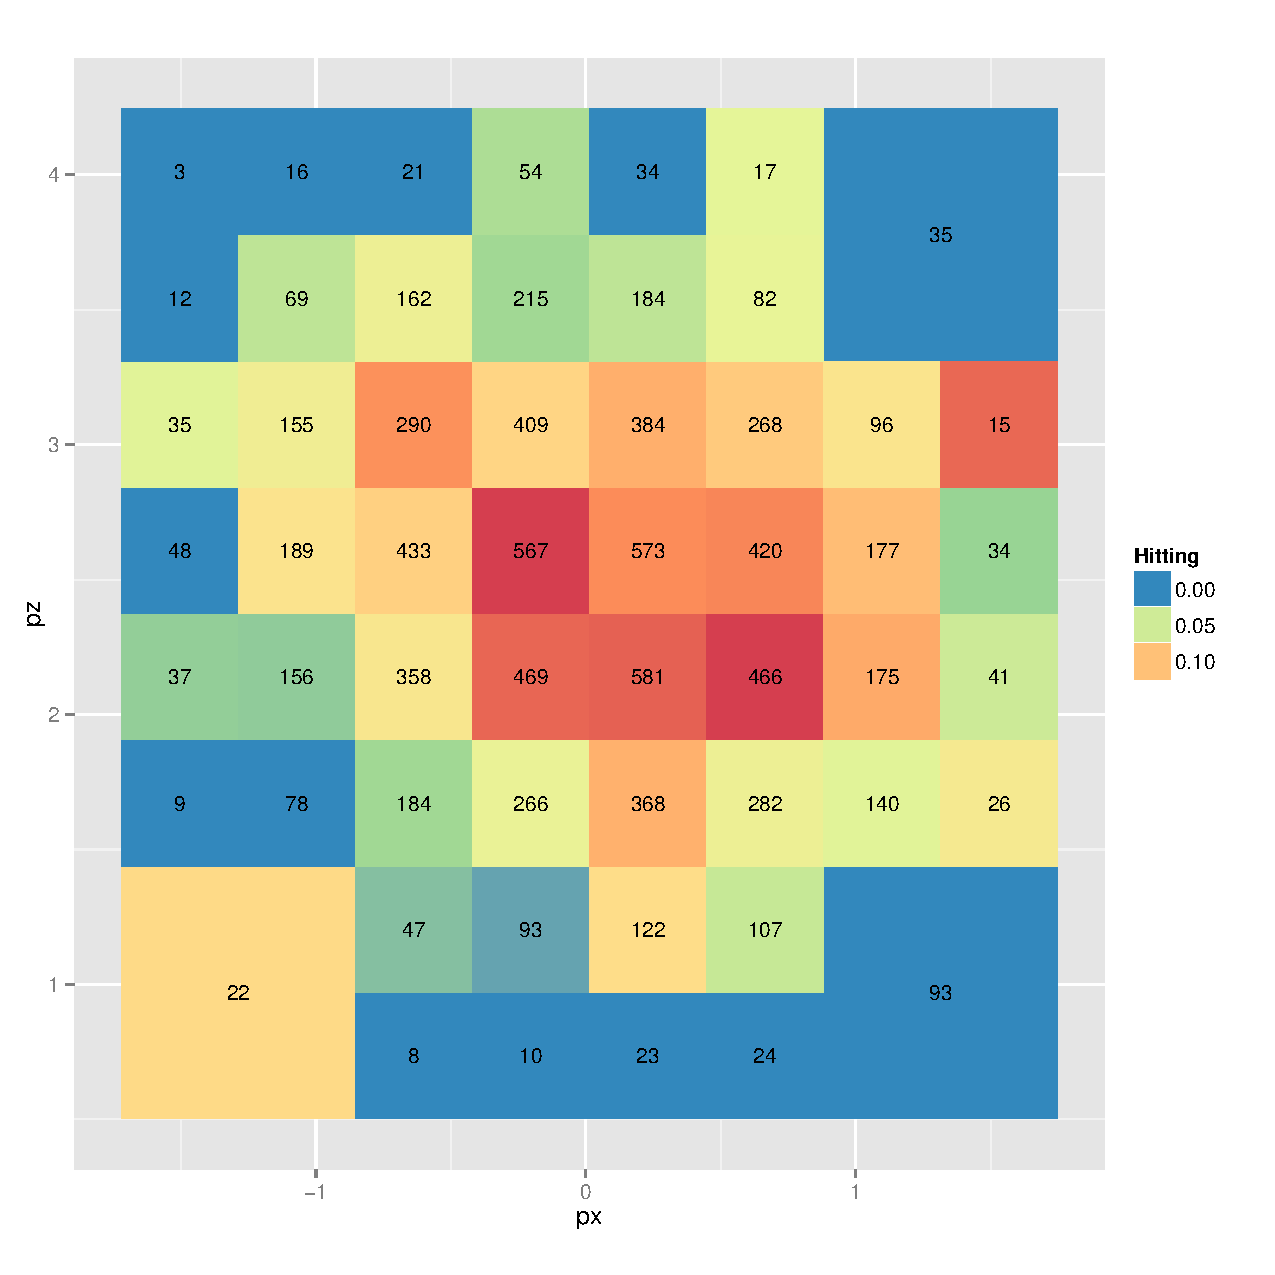
\includegraphics[scale=.2]{Images/Chapter8x8_100.pdf}
      	\caption{...(these images, and others, need labels: (A) (B) (C) etc)}
\end{figure} 
For this reason the bottom left heat maps in Figures 7 and 8, shown in Figure 9, differ in the number of boxes of each size, and the total number of boxes. This divergence continues at the next iteration, where the stopping rule $n_{b} < 100$ requires 28 box subdivisions in Figure 8, map three; and $n_{b} < 200$ gives 16 box subdivisions in Figure 7, map three.

% *Alix: ``I wonder if there's any literature on the physics from a hitter's perspective in terms of how small a difference in location is even detectable.

% *Alix: ``Great start Chris. --> need to add more about how one would now interpret the ``best'' empirical heat map.

% \subsection{Appendix: VarResHM, An R Package}

% 
% \bibliography{Baseball}
% 
% \end{document}